%%%%%%%%%%%%%%%%%%%%%%%%%%%%%%%%%%%%%%%%%
% Masters/Doctoral Thesis
% LaTeX Template
% Version 2.3 (25/3/16)
%
% This template has been downloaded from:
% http://www.LaTeXTemplates.com
%
% Version 2.x major modifications by:
% Vel (vel@latextemplates.com)
%
% This template is based on a template by:
% Steve Gunn (http://users.ecs.soton.ac.uk/srg/softwaretools/document/templates/)
% Sunil Patel (http://www.sunilpatel.co.uk/thesis-template/)
%
% Template license:
% CC BY-NC-SA 3.0 (http://creativecommons.org/licenses/by-nc-sa/3.0/)
%
%%%%%%%%%%%%%%%%%%%%%%%%%%%%%%%%%%%%%%%%%

%----------------------------------------------------------------------------------------
%	PACKAGES AND OTHER DOCUMENT CONFIGURATIONS
%----------------------------------------------------------------------------------------

\documentclass[
11pt, % The default document font size, options: 10pt, 11pt, 12pt
%oneside, % Two side (alternating margins) for binding by default, uncomment to switch to one side
%chapterinoneline,% Have the chapter title next to the number in one single line
english, % ngerman for German
singlespacing, % Single line spacing, alternatives: onehalfspacing or doublespacing
%draft, % Uncomment to enable draft mode (no pictures, no links, overfull hboxes indicated)
%nolistspacing, % If the document is onehalfspacing or doublespacing, uncomment this to set spacing in lists to single
%liststotoc, % Uncomment to add the list of figures/tables/etc to the table of contents
%toctotoc, % Uncomment to add the main table of contents to the table of contents
parskip, % Uncomment to add space between paragraphs
%nohyperref, % Uncomment to not load the hyperref package
headsepline, % Uncomment to get a line under the header
]{MastersDoctoralThesis} % The class file specifying the document structure

\usepackage[utf8]{inputenc} % Required for inputting international characters
\usepackage[T1]{fontenc} % Output font encoding for international characters

\usepackage{palatino} % Use the Palatino font by default

\usepackage[backend=bibtex,natbib=true]{biblatex} % Use the bibtex backend with the authoryear citation style (which resembles APA)

\addbibresource{mpotr.bib} % The filename of the bibliography

\usepackage[autostyle=true]{csquotes} % Required to generate language-dependent quotes in the bibliography

\usepackage{amsmath}
\usepackage{float}
\usepackage[algoruled]{algorithm2e}
\usepackage{tikz}
\usepackage{listings}
\usepackage{bytefield}
\usepackage{enumitem}
\usepackage[keys, operators]{cryptocode}
\usepackage{subcaption}


%Define the myinput macro for algorithm2e
\newlength\mylen
\newcommand\KwExtraIn[1]{%
        \settowidth\mylen{\KwIn{}}%
        \setlength\hangindent{\mylen}%
        \hspace*{\mylen}#1\\}

\newcommand\NextYear{%
  \advance\year by 1 \the\year\advance\year by -1}
\newcommand\PrevYear{%
  \advance\year by -1 \the\year\advance\year by 1}


%----------------------------------------------------------------------------------------
%	MARGIN SETTINGS
%----------------------------------------------------------------------------------------

\geometry{
	paper=a4paper, % Change to letterpaper for US letter
	inner=2.5cm, % Inner margin
	outer=3.8cm, % Outer margin
	bindingoffset=2cm, % Binding offset
	top=1.5cm, % Top margin
	bottom=1.5cm, % Bottom margin
	%showframe,% show how the type block is set on the page
}

%----------------------------------------------------------------------------------------
%	THESIS INFORMATION
%----------------------------------------------------------------------------------------

\thesistitle{Implementation of a Multi-party Off-the-Record messaging protocol} % Your thesis title, this is used in the title and abstract, print it elsewhere with \ttitle
\supervisor{Aristides \textsc{Pagourtzis}} % Your supervisor's name, this is used in the title page, print it elsewhere with \supname
\examiner{} % Your examiner's name, this is not currently used anywhere in the template, print it elsewhere with \examname
\degree{Master of Engineering} % Your degree name, this is used in the title page and abstract, print it elsewhere with \degreename
\author{\mbox{Konsantinos \textsc{Andrikopoulos}}, Dimitrios \textsc{Kolotouros}} % Your name, this is used in the title page and abstract, print it elsewhere with \authorname
\addresses{} % Your address, this is not currently used anywhere in the template, print it elsewhere with \addressname

\subject{Cryptography} % Your subject area, this is not currently used anywhere in the template, print it elsewhere with \subjectname
\keywords{Privacy, Group Messaging, Authentication, Enrytpion, Trancript Consistency, End to End, Surveillance} % Keywords for your thesis, this is not currently used anywhere in the template, print it elsewhere with \keywordnames
\university{\href{http://www.ntua.gr}{National Technical University of Athens}} % Your university's name and URL, this is used in the title page and abstract, print it elsewhere with \univname
\department{\href{http://department.university.com}{School of Electrical and Computer Engineering}} % Your department's name and URL, this is used in the title page and abstract, print it elsewhere with \deptname
\group{\href{http://researchgroup.university.com}{asdf}} % Your research group's name and URL, this is used in the title page, print it elsewhere with \groupname
\faculty{\href{http://faculty.university.com}{Faculty Name}} % Your faculty's name and URL, this is used in the title page and abstract, print it elsewhere with \facname


\hypersetup{pdftitle=\ttitle} % Set the PDF's title to your title
\hypersetup{pdfauthor=\authorname} % Set the PDF's author to your name
\hypersetup{pdfkeywords=\keywordnames} % Set the PDF's keywords to your keywords

\begin{document}

\frontmatter % Use roman page numbering style (i, ii, iii, iv...) for the pre-content pages

\pagestyle{plain} % Default to the plain heading style until the thesis style is called for the body content

%----------------------------------------------------------------------------------------
%	TITLE PAGE
%----------------------------------------------------------------------------------------

\begin{titlepage}
\begin{center}

{\scshape\LARGE \univname\par}\vspace{1.5cm} % University name
\textsc{\Large Diploma Thesis}\\[0.5cm] % Thesis type

\HRule \\[0.4cm] % Horizontal line
{\huge \bfseries \ttitle\par}\vspace{0.4cm} % Thesis title
\HRule \\[1.5cm] % Horizontal line

\begin{minipage}[t]{0.49\textwidth}
\begin{flushleft} \large
\emph{Authors:}\\
\href{http://www.johnsmith.com}{\authorname} \\ % Author name - remove the \href bracket to remove the link
\end{flushleft}
\end{minipage}
\begin{minipage}[t]{0.49\textwidth}
\begin{flushright} \large
\emph{Supervisor:} \\
\href{http://www.jamessmith.com}{\supname} % Supervisor name - remove the \href bracket to remove the link
\end{flushright}
\end{minipage}\\[3cm]

\large \textit{A thesis submitted in fulfillment of the requirements\\ for the degree of \degreename}\\[0.3cm] % University requirement text
\textit{in the}\\[0.4cm]
\deptname\\[2cm] % Research group name and department name

\vfill

{\large \today}\\[4cm] % Date
%\includegraphics{Logo} % University/department logo - uncomment to place it

\vfill
\end{center}
\end{titlepage}

%----------------------------------------------------------------------------------------
%	DECLARATION PAGE
%----------------------------------------------------------------------------------------

%\begin{declaration}
%\addchaptertocentry{\authorshipname}
%
%\noindent We, \authorname, declare that this thesis titled, \enquote{\ttitle} and the work presented in it are our own. We confirm that:
%
%\begin{itemize}
%\item This work was done wholly or mainly while in candidature for a research degree at this University.
%\item Where any part of this thesis has previously been submitted for a degree or any other qualification at this University or any other institution, this has been clearly stated.
%\item Where We have consulted the published work of others, this is always clearly attributed.
%\item Where We have quoted from the work of others, the source is always given. With the exception of such quotations, this thesis is entirely our own work.
%\item We have acknowledged all main sources of help.
%\item Where the thesis is based on work done by us jointly with others, I have made clear exactly what was done by others and what We have contributed ourselves.\\
%\end{itemize}
%
%\noindent Signed:\\
%\rule[0.5em]{25em}{0.5pt} % This prints a line for the signature
%
%\noindent Date:\\
%\rule[0.5em]{25em}{0.5pt} % This prints a line to write the date
%\end{declaration}

\cleardoublepage

%----------------------------------------------------------------------------------------
%	QUOTATION PAGE
%----------------------------------------------------------------------------------------

\vspace*{0.2\textheight}

\noindent\enquote{\itshape Thanks to my solid academic training, today I can write hundreds of words on virtually any topic without possessing a shred of information, which is how I got a good job in journalism.}\bigbreak

\hfill Dave Barry

%----------------------------------------------------------------------------------------
%	ABSTRACT PAGE
%----------------------------------------------------------------------------------------

\begin{abstract}
\addchaptertocentry{\abstractname} % Add the abstract to the table of contents

In a world where the need for easy instant communication must overcome the threat of constant surveillance, end-to-end encryption has become a necessity.
While some protocols enable end-to-end encryption for two parties, there are limited solutions for multiparty end-to-end encryption, particularly for desktop applications.
In this paper we describe the first implementation of mpOTR, the multiparty OTR protocol.
mpOTR achieves confidentiality, authenticity, forward secrecy, deniability, and basic consensus.
The existing theoretical introduction of mpOTR treats the undrelying subprotocols as black boxes and does not describe them in detail.
Our contributions are the complete description of the mpOTR protocol including every subprotocol detail and the first implementation of mpOTR.
Our implementation is a production-grade open source extension of the existing libotr library accompanied by a Pidgin plugin written in C.

  \vspace*{\fill}

{\bf Keywords}: \keywordnames
\end{abstract}

%----------------------------------------------------------------------------------------
%	ACKNOWLEDGEMENTS
%----------------------------------------------------------------------------------------

\begin{acknowledgements}
\addchaptertocentry{\acknowledgementname} % Add the acknowledgements to the table of contents

The acknowledgments and the people to thank go here, don't forget to include your project advisor\ldots

\end{acknowledgements}

%----------------------------------------------------------------------------------------
%	LIST OF CONTENTS/FIGURES/TABLES PAGES
%----------------------------------------------------------------------------------------

\tableofcontents % Prints the main table of contents

\listoffigures % Prints the list of figures

\listoftables % Prints the list of tables

%----------------------------------------------------------------------------------------
%	ABBREVIATIONS
%----------------------------------------------------------------------------------------

\begin{abbreviations}{ll} % Include a list of abbreviations (a table of two columns)

\textbf{LAH} & \textbf{L}ist \textbf{A}bbreviations \textbf{H}ere\\
\textbf{WSF} & \textbf{W}hat (it) \textbf{S}tands \textbf{F}or\\

\end{abbreviations}

%----------------------------------------------------------------------------------------
%	SYMBOLS
%----------------------------------------------------------------------------------------

\begin{symbols}{ll} % Include a list of Symbols (a three column table)

  $AES_{CTR}$   & AES block cipher in counter mode \\
  $\mathcal{O}$ & Security Adversary \\
  $\mathcal{M}$ & Privacy Adversary \\
  $\mathcal{T}$ & Consensus Adversary \\
  $H$           & A hash function \\
  $\oplus$      & The XOR operation \\
  $\odot$ or $\diamond$ & A generic operation \\

%Symbol & Name & Unit \\

\addlinespace % Gap to separate the Roman symbols from the Greek

\end{symbols}

%----------------------------------------------------------------------------------------
%	DEDICATION
%----------------------------------------------------------------------------------------

\dedicatory{For/Dedicated to/To my\ldots}

%----------------------------------------------------------------------------------------
%	THESIS CONTENT - CHAPTERS
%----------------------------------------------------------------------------------------

\mainmatter % Begin numeric (1,2,3...) page numbering

\pagestyle{thesis} % Return the page headers back to the "thesis" style

% Include the chapters of the thesis as separate files from the Chapters folder
% Uncomment the lines as you write the chapters

%% Chapter 1

\chapter{Chapter Title Here} % Main chapter title

\label{Chapter1} % For referencing the chapter elsewhere, use \ref{Chapter1}

%----------------------------------------------------------------------------------------

% Define some commands to keep the formatting separated from the content
\newcommand{\keyword}[1]{\textbf{#1}}
\newcommand{\tabhead}[1]{\textbf{#1}}
\newcommand{\code}[1]{\texttt{#1}}
\newcommand{\file}[1]{\texttt{\bfseries#1}}
\newcommand{\option}[1]{\texttt{\itshape#1}}

%----------------------------------------------------------------------------------------

\section{Welcome and Thank You}
Welcome to this \LaTeX{} Thesis Template \cite{mpotr}, a beautiful and easy to use template for writing a thesis using the \LaTeX{} typesetting system.

If you are writing a thesis (or will be in the future) and its subject is technical or mathematical (though it doesn't have to be), then creating it in \LaTeX{} is highly recommended as a way to make sure you can just get down to the essential writing without having to worry over formatting or wasting time arguing with your word processor.

\LaTeX{} is easily able to professionally typeset documents that run to hundreds or thousands of pages long. With simple mark-up commands, it automatically sets out the table of contents, margins, page headers and footers and keeps the formatting consistent and beautiful. One of its main strengths is the way it can easily typeset mathematics, even \emph{heavy} mathematics. Even if those equations are the most horribly twisted and most difficult mathematical problems that can only be solved on a super-computer, you can at least count on \LaTeX{} to make them look stunning.

%----------------------------------------------------------------------------------------

\section{Learning \LaTeX{}}

\LaTeX{} is not a \textsc{wysiwyg} (What You See is What You Get) program, unlike word processors such as Microsoft Word or Apple's Pages. Instead, a document written for \LaTeX{} is actually a simple, plain text file that contains \emph{no formatting}. You tell \LaTeX{} how you want the formatting in the finished document by writing in simple commands amongst the text, for example, if I want to use \emph{italic text for emphasis}, I write the \verb|\emph{text}| command and put the text I want in italics in between the curly braces. This means that \LaTeX{} is a \enquote{mark-up} language, very much like HTML.

\subsection{A (not so short) Introduction to \LaTeX{}}

If you are new to \LaTeX{}, there is a very good eBook -- freely available online as a PDF file -- called, \enquote{The Not So Short Introduction to \LaTeX{}}. The book's title is typically shortened to just \emph{lshort}. You can download the latest version (as it is occasionally updated) from here:
\url{http://www.ctan.org/tex-archive/info/lshort/english/lshort.pdf}

It is also available in several other languages. Find yours from the list on this page: \url{http://www.ctan.org/tex-archive/info/lshort/}

It is recommended to take a little time out to learn how to use \LaTeX{} by creating several, small `test' documents, or having a close look at several templates on:\\
\url{http://www.LaTeXTemplates.com}\\
Making the effort now means you're not stuck learning the system when what you \emph{really} need to be doing is writing your thesis.

\subsection{A Short Math Guide for \LaTeX{}}

If you are writing a technical or mathematical thesis, then you may want to read the document by the AMS (American Mathematical Society) called, \enquote{A Short Math Guide for \LaTeX{}}. It can be found online here:
\url{http://www.ams.org/tex/amslatex.html}
under the \enquote{Additional Documentation} section towards the bottom of the page.

\subsection{Common \LaTeX{} Math Symbols}
There are a multitude of mathematical symbols available for \LaTeX{} and it would take a great effort to learn the commands for them all. The most common ones you are likely to use are shown on this page:
\url{http://www.sunilpatel.co.uk/latex-type/latex-math-symbols/}

You can use this page as a reference or crib sheet, the symbols are rendered as large, high quality images so you can quickly find the \LaTeX{} command for the symbol you need.

\subsection{\LaTeX{} on a Mac}

The \LaTeX{} distribution is available for many systems including Windows, Linux and Mac OS X. The package for OS X is called MacTeX and it contains all the applications you need -- bundled together and pre-customized -- for a fully working \LaTeX{} environment and work flow.

MacTeX includes a custom dedicated \LaTeX{} editor called TeXShop for writing your `\file{.tex}' files and BibDesk: a program to manage your references and create your bibliography section just as easily as managing songs and creating playlists in iTunes.

%----------------------------------------------------------------------------------------

\section{Getting Started with this Template}

If you are familiar with \LaTeX{}, then you should explore the directory structure of the template and then proceed to place your own information into the \emph{THESIS INFORMATION} block of the \file{main.tex} file. You can then modify the rest of this file to your unique specifications based on your degree/university. Section \ref{FillingFile} on page \pageref{FillingFile} will help you do this. Make sure you also read section \ref{ThesisConventions} about thesis conventions to get the most out of this template.

If you are new to \LaTeX{} it is recommended that you carry on reading through the rest of the information in this document.

Before you begin using this template you should ensure that its style complies with the thesis style guidelines imposed by your institution. In most cases this template style and layout will be suitable. If it is not, it may only require a small change to bring the template in line with your institution's recommendations. These modifications will need to be done on the \file{MastersDoctoralThesis.cls} file.

\subsection{About this Template}

This \LaTeX{} Thesis Template is originally based and created around a \LaTeX{} style file created by Steve R.\ Gunn from the University of Southampton (UK), department of Electronics and Computer Science. You can find his original thesis style file at his site, here:
\url{http://www.ecs.soton.ac.uk/~srg/softwaretools/document/templates/}

Steve's \file{ecsthesis.cls} was then taken by Sunil Patel who modified it by creating a skeleton framework and folder structure to place the thesis files in. The resulting template can be found on Sunil's site here:
\url{http://www.sunilpatel.co.uk/thesis-template}

Sunil's template was made available through \url{http://www.LaTeXTemplates.com} where it was modified many times based on user requests and questions. Version 2.0 and onwards of this template represents a major modification to Sunil's template and is, in fact, hardly recognisable. The work to make version 2.0 possible was carried out by \href{mailto:vel@latextemplates.com}{Vel} and Johannes Böttcher.

%----------------------------------------------------------------------------------------

\section{What this Template Includes}

\subsection{Folders}

This template comes as a single zip file that expands out to several files and folders. The folder names are mostly self-explanatory:

\keyword{Appendices} -- this is the folder where you put the appendices. Each appendix should go into its own separate \file{.tex} file. An example and template are included in the directory.

\keyword{Chapters} -- this is the folder where you put the thesis chapters. A thesis usually has about six chapters, though there is no hard rule on this. Each chapter should go in its own separate \file{.tex} file and they can be split as:
\begin{itemize}
\item Chapter 1: Introduction to the thesis topic
\item Chapter 2: Background information and theory
\item Chapter 3: (Laboratory) experimental setup
\item Chapter 4: Details of experiment 1
\item Chapter 5: Details of experiment 2
\item Chapter 6: Discussion of the experimental results
\item Chapter 7: Conclusion and future directions
\end{itemize}
This chapter layout is specialised for the experimental sciences.

\keyword{Figures} -- this folder contains all figures for the thesis. These are the final images that will go into the thesis document.

\subsection{Files}

Included are also several files, most of them are plain text and you can see their contents in a text editor. After initial compilation, you will see that more auxiliary files are created by \LaTeX{} or BibTeX and which you don't need to delete or worry about:

\keyword{example.bib} -- this is an important file that contains all the bibliographic information and references that you will be citing in the thesis for use with BibTeX. You can write it manually, but there are reference manager programs available that will create and manage it for you. Bibliographies in \LaTeX{} are a large subject and you may need to read about BibTeX before starting with this. Many modern reference managers will allow you to export your references in BibTeX format which greatly eases the amount of work you have to do.

\keyword{MastersDoctoralThesis.cls} -- this is an important file. It is the class file that tells \LaTeX{} how to format the thesis.

\keyword{main.pdf} -- this is your beautifully typeset thesis (in the PDF file format) created by \LaTeX{}. It is supplied in the PDF with the template and after you compile the template you should get an identical version.

\keyword{main.tex} -- this is an important file. This is the file that you tell \LaTeX{} to compile to produce your thesis as a PDF file. It contains the framework and constructs that tell \LaTeX{} how to layout the thesis. It is heavily commented so you can read exactly what each line of code does and why it is there. After you put your own information into the \emph{THESIS INFORMATION} block -- you have now started your thesis!

Files that are \emph{not} included, but are created by \LaTeX{} as auxiliary files include:

\keyword{main.aux} -- this is an auxiliary file generated by \LaTeX{}, if it is deleted \LaTeX{} simply regenerates it when you run the main \file{.tex} file.

\keyword{main.bbl} -- this is an auxiliary file generated by BibTeX, if it is deleted, BibTeX simply regenerates it when you run the \file{main.aux} file. Whereas the \file{.bib} file contains all the references you have, this \file{.bbl} file contains the references you have actually cited in the thesis and is used to build the bibliography section of the thesis.

\keyword{main.blg} -- this is an auxiliary file generated by BibTeX, if it is deleted BibTeX simply regenerates it when you run the main \file{.aux} file.

\keyword{main.lof} -- this is an auxiliary file generated by \LaTeX{}, if it is deleted \LaTeX{} simply regenerates it when you run the main \file{.tex} file. It tells \LaTeX{} how to build the \emph{List of Figures} section.

\keyword{main.log} -- this is an auxiliary file generated by \LaTeX{}, if it is deleted \LaTeX{} simply regenerates it when you run the main \file{.tex} file. It contains messages from \LaTeX{}, if you receive errors and warnings from \LaTeX{}, they will be in this \file{.log} file.

\keyword{main.lot} -- this is an auxiliary file generated by \LaTeX{}, if it is deleted \LaTeX{} simply regenerates it when you run the main \file{.tex} file. It tells \LaTeX{} how to build the \emph{List of Tables} section.

\keyword{main.out} -- this is an auxiliary file generated by \LaTeX{}, if it is deleted \LaTeX{} simply regenerates it when you run the main \file{.tex} file.

So from this long list, only the files with the \file{.bib}, \file{.cls} and \file{.tex} extensions are the most important ones. The other auxiliary files can be ignored or deleted as \LaTeX{} and BibTeX will regenerate them.

%----------------------------------------------------------------------------------------

\section{Filling in Your Information in the \file{main.tex} File}\label{FillingFile}

You will need to personalise the thesis template and make it your own by filling in your own information. This is done by editing the \file{main.tex} file in a text editor or your favourite LaTeX environment.

Open the file and scroll down to the second large block titled \emph{THESIS INFORMATION} where you can see the entries for \emph{University Name}, \emph{Department Name}, etc \ldots

Fill out the information about yourself, your group and institution. You can also insert web links, if you do, make sure you use the full URL, including the \code{http://} for this. If you don't want these to be linked, simply remove the \verb|\href{url}{name}| and only leave the name.

When you have done this, save the file and recompile \code{main.tex}. All the information you filled in should now be in the PDF, complete with web links. You can now begin your thesis proper!

%----------------------------------------------------------------------------------------

\section{The \code{main.tex} File Explained}

The \file{main.tex} file contains the structure of the thesis. There are plenty of written comments that explain what pages, sections and formatting the \LaTeX{} code is creating. Each major document element is divided into commented blocks with titles in all capitals to make it obvious what the following bit of code is doing. Initially there seems to be a lot of \LaTeX{} code, but this is all formatting, and it has all been taken care of so you don't have to do it.

Begin by checking that your information on the title page is correct. For the thesis declaration, your institution may insist on something different than the text given. If this is the case, just replace what you see with what is required in the \emph{DECLARATION PAGE} block.

Then comes a page which contains a funny quote. You can put your own, or quote your favourite scientist, author, person, and so on. Make sure to put the name of the person who you took the quote from.

Following this is the abstract page which summarises your work in a condensed way and can almost be used as a standalone document to describe what you have done. The text you write will cause the heading to move up so don't worry about running out of space.

Next come the acknowledgements. On this page, write about all the people who you wish to thank (not forgetting parents, partners and your advisor/supervisor).

The contents pages, list of figures and tables are all taken care of for you and do not need to be manually created or edited. The next set of pages are more likely to be optional and can be deleted since they are for a more technical thesis: insert a list of abbreviations you have used in the thesis, then a list of the physical constants and numbers you refer to and finally, a list of mathematical symbols used in any formulae. Making the effort to fill these tables means the reader has a one-stop place to refer to instead of searching the internet and references to try and find out what you meant by certain abbreviations or symbols.

The list of symbols is split into the Roman and Greek alphabets. Whereas the abbreviations and symbols ought to be listed in alphabetical order (and this is \emph{not} done automatically for you) the list of physical constants should be grouped into similar themes.

The next page contains a one line dedication. Who will you dedicate your thesis to?

Finally, there is the block where the chapters are included. Uncomment the lines (delete the \code{\%} character) as you write the chapters. Each chapter should be written in its own file and put into the \emph{Chapters} folder and named \file{Chapter1}, \file{Chapter2}, etc\ldots Similarly for the appendices, uncomment the lines as you need them. Each appendix should go into its own file and placed in the \emph{Appendices} folder.

After the preamble, chapters and appendices finally comes the bibliography. The bibliography style (called \option{authoryear}) is used for the bibliography and is a fully featured style that will even include links to where the referenced paper can be found online. Do not underestimate how grateful your reader will be to find that a reference to a paper is just a click away. Of course, this relies on you putting the URL information into the BibTeX file in the first place.

%----------------------------------------------------------------------------------------

\section{Thesis Features and Conventions}\label{ThesisConventions}

To get the best out of this template, there are a few conventions that you may want to follow.

One of the most important (and most difficult) things to keep track of in such a long document as a thesis is consistency. Using certain conventions and ways of doing things (such as using a Todo list) makes the job easier. Of course, all of these are optional and you can adopt your own method.

\subsection{Printing Format}

This thesis template is designed for double sided printing (i.e. content on the front and back of pages) as most theses are printed and bound this way. Switching to one sided printing is as simple as uncommenting the \option{oneside} option of the \code{documentclass} command at the top of the \file{main.tex} file. You may then wish to adjust the margins to suit specifications from your institution.

The headers for the pages contain the page number on the outer side (so it is easy to flick through to the page you want) and the chapter name on the inner side.

The text is set to 11 point by default with single line spacing, again, you can tune the text size and spacing should you want or need to using the options at the very start of \file{main.tex}. The spacing can be changed similarly by replacing the \option{singlespacing} with \option{onehalfspacing} or \option{doublespacing}.

\subsection{Using US Letter Paper}

The paper size used in the template is A4, which is the standard size in Europe. If you are using this thesis template elsewhere and particularly in the United States, then you may have to change the A4 paper size to the US Letter size. This can be done in the margins settings section in \file{main.tex}.

Due to the differences in the paper size, the resulting margins may be different to what you like or require (as it is common for institutions to dictate certain margin sizes). If this is the case, then the margin sizes can be tweaked by modifying the values in the same block as where you set the paper size. Now your document should be set up for US Letter paper size with suitable margins.

\subsection{References}

The \code{biblatex} package is used to format the bibliography and inserts references such as this one \parencite{Reference1}. The options used in the \file{main.tex} file mean that the in-text citations of references are formatted with the author(s) listed with the date of the publication. Multiple references are separated by semicolons (e.g. \parencite{Reference2, Reference1}) and references with more than three authors only show the first author with \emph{et al.} indicating there are more authors (e.g. \parencite{Reference3}). This is done automatically for you. To see how you use references, have a look at the \file{Chapter1.tex} source file. Many reference managers allow you to simply drag the reference into the document as you type.

Scientific references should come \emph{before} the punctuation mark if there is one (such as a comma or period). The same goes for footnotes\footnote{Such as this footnote, here down at the bottom of the page.}. You can change this but the most important thing is to keep the convention consistent throughout the thesis. Footnotes themselves should be full, descriptive sentences (beginning with a capital letter and ending with a full stop). The APA6 states: \enquote{Footnote numbers should be superscripted, [...], following any punctuation mark except a dash.} The Chicago manual of style states: \enquote{A note number should be placed at the end of a sentence or clause. The number follows any punctuation mark except the dash, which it precedes. It follows a closing parenthesis.}

The bibliography is typeset with references listed in alphabetical order by the first author's last name. This is similar to the APA referencing style. To see how \LaTeX{} typesets the bibliography, have a look at the very end of this document (or just click on the reference number links in in-text citations).

\subsubsection{A Note on bibtex}

The bibtex backend used in the template by default does not correctly handle unicode character encoding (i.e. "international" characters). You may see a warning about this in the compilation log and, if your references contain unicode characters, they may not show up correctly or at all. The solution to this is to use the biber backend instead of the outdated bibtex backend. This is done by finding this in \file{main.tex}: \option{backend=bibtex} and changing it to \option{backend=biber}. You will then need to delete all auxiliary BibTeX files and navigate to the template directory in your terminal (command prompt). Once there, simply type \code{biber main} and biber will compile your bibliography. You can then compile \file{main.tex} as normal and your bibliography will be updated. An alternative is to set up your LaTeX editor to compile with biber instead of bibtex, see \href{http://tex.stackexchange.com/questions/154751/biblatex-with-biber-configuring-my-editor-to-avoid-undefined-citations/}{here} for how to do this for various editors.

\subsection{Tables}

Tables are an important way of displaying your results, below is an example table which was generated with this code:

{\small
\begin{verbatim}
\begin{table}
\caption{The effects of treatments X and Y on the four groups studied.}
\label{tab:treatments}
\centering
\begin{tabular}{l l l}
\toprule
\tabhead{Groups} & \tabhead{Treatment X} & \tabhead{Treatment Y} \\
\midrule
1 & 0.2 & 0.8\\
2 & 0.17 & 0.7\\
3 & 0.24 & 0.75\\
4 & 0.68 & 0.3\\
\bottomrule\\
\end{tabular}
\end{table}
\end{verbatim}
}

\begin{table}
\caption{The effects of treatments X and Y on the four groups studied.}
\label{tab:treatments}
\centering
\begin{tabular}{l l l}
\toprule
\tabhead{Groups} & \tabhead{Treatment X} & \tabhead{Treatment Y} \\
\midrule
1 & 0.2 & 0.8\\
2 & 0.17 & 0.7\\
3 & 0.24 & 0.75\\
4 & 0.68 & 0.3\\
\bottomrule\\
\end{tabular}
\end{table}

You can reference tables with \verb|\ref{<label>}| where the label is defined within the table environment. See \file{Chapter1.tex} for an example of the label and citation (e.g. Table~\ref{tab:treatments}).

\subsection{Figures}

There will hopefully be many figures in your thesis (that should be placed in the \emph{Figures} folder). The way to insert figures into your thesis is to use a code template like this:
\begin{verbatim}
\begin{figure}
\centering
\includegraphics{Figures/Electron}
\decoRule
\caption[An Electron]{An electron (artist's impression).}
\label{fig:Electron}
\end{figure}
\end{verbatim}
Also look in the source file. Putting this code into the source file produces the picture of the electron that you can see in the figure below.

\begin{figure}[h]
\centering
\includegraphics{Figures/Electron}
\decoRule
\caption[An Electron]{An electron (artist's impression).}
\label{fig:Electron}
\end{figure}

Sometimes figures don't always appear where you write them in the source. The placement depends on how much space there is on the page for the figure. Sometimes there is not enough room to fit a figure directly where it should go (in relation to the text) and so \LaTeX{} puts it at the top of the next page. Positioning figures is the job of \LaTeX{} and so you should only worry about making them look good!

Figures usually should have captions just in case you need to refer to them (such as in Figure~\ref{fig:Electron}). The \verb|\caption| command contains two parts, the first part, inside the square brackets is the title that will appear in the \emph{List of Figures}, and so should be short. The second part in the curly brackets should contain the longer and more descriptive caption text.

The \verb|\decoRule| command is optional and simply puts an aesthetic horizontal line below the image. If you do this for one image, do it for all of them.

\LaTeX{} is capable of using images in pdf, jpg and png format.

\subsection{Typesetting mathematics}

If your thesis is going to contain heavy mathematical content, be sure that \LaTeX{} will make it look beautiful, even though it won't be able to solve the equations for you.

The \enquote{Not So Short Introduction to \LaTeX} (available on \href{http://www.ctan.org/tex-archive/info/lshort/english/lshort.pdf}{CTAN}) should tell you everything you need to know for most cases of typesetting mathematics. If you need more information, a much more thorough mathematical guide is available from the AMS called, \enquote{A Short Math Guide to \LaTeX} and can be downloaded from:
\url{ftp://ftp.ams.org/pub/tex/doc/amsmath/short-math-guide.pdf}

There are many different \LaTeX{} symbols to remember, luckily you can find the most common symbols in \href{http://ctan.org/pkg/comprehensive}{The Comprehensive \LaTeX~Symbol List}.

You can write an equation, which is automatically given an equation number by \LaTeX{} like this:
\begin{verbatim}
\begin{equation}
E = mc^{2}
\label{eqn:Einstein}
\end{equation}
\end{verbatim}

This will produce Einstein's famous energy-matter equivalence equation:
\begin{equation}
E = mc^{2}
\label{eqn:Einstein}
\end{equation}

All equations you write (which are not in the middle of paragraph text) are automatically given equation numbers by \LaTeX{}. If you don't want a particular equation numbered, use the unnumbered form:
\begin{verbatim}
\[ a^{2}=4 \]
\end{verbatim}

%----------------------------------------------------------------------------------------

\section{Sectioning and Subsectioning}

You should break your thesis up into nice, bite-sized sections and subsections. \LaTeX{} automatically builds a table of Contents by looking at all the \verb|\chapter{}|, \verb|\section{}|  and \verb|\subsection{}| commands you write in the source.

The Table of Contents should only list the sections to three (3) levels. A \verb|chapter{}| is level zero (0). A \verb|\section{}| is level one (1) and so a \verb|\subsection{}| is level two (2). In your thesis it is likely that you will even use a \verb|subsubsection{}|, which is level three (3). The depth to which the Table of Contents is formatted is set within \file{MastersDoctoralThesis.cls}. If you need this changed, you can do it in \file{main.tex}.

%----------------------------------------------------------------------------------------

\section{In Closing}

You have reached the end of this mini-guide. You can now rename or overwrite this pdf file and begin writing your own \file{Chapter1.tex} and the rest of your thesis. The easy work of setting up the structure and framework has been taken care of for you. It's now your job to fill it out!

Good luck and have lots of fun!

\begin{flushright}
Guide written by ---\\
Sunil Patel: \href{http://www.sunilpatel.co.uk}{www.sunilpatel.co.uk}\\
Vel: \href{http://www.LaTeXTemplates.com}{LaTeXTemplates.com}
\end{flushright}

\chapter{Introduction}

\label{chapter:introduction}

\newcommand{\dhname}{Diffie--Hellman }
\newcommand{\tdhname}{Triple Diffie--Hellman }


%--------------------------------------------

\section{Motivation}
Not much time has passed since Edward Snowden revealed the plans that a certain intelligence agency has for the internet. While the world had always been suspecting that the various 3-letter agencies had the capability of controlling the network at a large scale, everybody was shocked with the confirmation of those suspicions.

In a world where the need for easy instant communication must overcome the threat of constant surveillance, end-to-end encryption has become a necessity. It's not a coincidence that digital privacy has come into focus during the last years. One after another companies advertise the utilization of encryption in their products. Apparently, Instant Messaging is the most favorable means of communication when it comes to end-to-end encryption.

One of the oldest and commonly used protocols that provides privacy in Instant Messaging is the Off-The-Record (OTR). OTR was initially introduced in a paper named "Off-the-Record Communication, or, Why Not To Use PGP" in 2004 \cite{otr} and later improved in \cite{otr_improvedauth}. It was named after the homonymous method of journal sourcing. The primary motivation behind OTR was to provide deniable authentication for the conversation participants while keeping conversations confidential, as in real-life private conversations. The protocol is implemented as a C library and a Pidgin plugin, a user study of which can be found in \cite{otr_userstudy}.

Unfortunately, OTR does only apply in a two-party setting, where only two participants are exchanging messages. However, multi-party chat rooms are also very prominent in everyday communications. A protocol providing the same privacy properties as OTR in a multi-party setting was theoritically described in the "Multi-party Off-the-Record Messaging" paper by I. Goldberg et al. in 2009 \cite{mpotr}. This protocol is called multi-party OTR (mpOTR). Although it's been around since 2009, no actual implementation of mpOTR existed until now.

\section{Our Contributions}
The existing theoretical introduction of mpOTR protocol in \cite{mpotr} treats the underlying subrotocols as black boxes and does not describe them in detail. More specifically, two underlying subprotocols are left unspecified, namely the deniable Authenticated Key Exchange (denAKE) and the Group Key Agreement (GKA). These sub-protocols play a key role in setting up the parameters needed for authentication and encryption.

We propose a full construction for the mpOTR Protocol. We specify every underlying sub-protocol. We also specify all the primitive algorithms used for several cryptographic functions, such as hashing, signing and encrypting. Finally, we propose a detailed low-level description of the protocol, including message structures, encoding, etc.

In addition, we provide the first implementation of mpOTR. Our implementation is a production-grade extension of the existing OTR library accompanied by a pidgin plugin, all writen in C. Both are open source projects, available in our github repositories\footnote{https://github.com/Mandragorian/libotr}\footnote{https://github.com/Mandragorian/pidgin\_otr}. We engineered our implementation in such a way that its security is easily reviewable, and, at the same time, facilitates the free software development model, where contributions in the source code are made from several independent authors.

\section{Outline}
In Chapter \ref{chapter:theoretic_background} we introduce some basic theoretic background. All the concepts, cryptographic primitives, and ideas presented there are essential building blocks of the mpOTR Protocol construction proposed in this thesis.

In Chapter \ref{chapter:threat_model} we specify the threat model of the mpOTR Protocol. We describe the different types of adversaries along with their goals. Then, we describe the goals of the mpOTR Protocol to achieve security against each type of adversary.

In Chapter \ref{chapter:protocol} we present our mpOTR Protocol construction. First, we specify the desirable privacy properties of mpOTR conversations and the underlying network setting. Then, we present a high-level overview of the protocol followed by a detailed description of every building block. Afterwards, we specify several technical details. Finally, we specify the exact structure of the messages exchanged in mpOTR.

In Chapter \ref{chapter:implementation} we present our actual implementation of mpOTR. We introduce  several design challenges and the relevant decisions. Then we present the design model of the mpOTR library. Finally, we specify the Application Programming Interface that our implementation offers to the IM applications in order to utilize mpOTR in group conversations.

In Chapter \ref{chapter:plugin} we present our modifications of the OTR pidgin plugin. We introduce the Graphical User interface and the workflow of a private group conversation.

In Chapter \ref{chapter:related_work} we present other protocols that utilize end-to-end encrpytion in multi-party context.

In Chapter \ref{chapter:future_work} we present several problems regarding specific parts of our mpOTR construction. While our construction is fully functional and secure, solving these problems would enhance the protocol’s privacy and/or usabilty. We fully describe each of them and suggest possible solutions.
\chapter{Theoretic Background}
\label{chapter:theoretic_background}

In this chapter we will present some basic theoretic background.
All the concepts, cryptographic primitives, and ideas presented here are essential building blocks of the protocol proposed in this thesis.
As a result before someone carries on forward in this document, she should first have a basic understanding of this chapter.

\section{Symmetric Encryption}

The idea of symmetric encryption is quite simple.
We suppose that there exists an algorithm called $E$, which takes two inputs.
One input is a secret, called the key, and the other is some data we would like to encrypt.

Another algorithm called $D$ again takes two inputs and is the reverse of $E$.
This means that if we call $D$ with inputs the output of $E$ under some key $k$, and $k$ itself, the output will be the plaintext data. This is shown in the below equation:

\[
  m = D(k, E(k, m))
\]

\section{Block Ciphers}

Block ciphers are a special case of symmetric encryption algorithms.
What makes them special is that they operate on a constant length block of data, hence the name.
While this constrain may appear very limiting, we will see that this is not the case.
In fact block ciphers have dominated the field of symmetric encryption.

The block cipher which is most commonly used is called AES, also known as Rijndael.
Its block size is 128 bits and depending on the AES version it has a key size of either 128, 192, or 256.

Exactly because AES is the most commonly used block cipher, it is also the most scrutinized and studied one.
Thus the crypto community is quite confident that AES is a secure construction, fully capable to be used for encrypted communications.

\section{Modes of Operation}

As we already stated, block ciphers operate on fixed chunks of data.
To overcome this limitation we need a mechanism so that we can break the plaintext in chunks of the cipher's block size, and then somehow apply the cipher in each chunk.
There are many modes of operation out there, but we will only talk about two of them.

One is called Electronic Code Book (ECB), and it is the naive solution that one can come up with when first tackling the problem at hand.
Suppose that we have a message $M$ which is a multiple of the block size.
We can then divide it into $n$ chunks $m_i$, each being one block in length:

\[
  M = m_1 \Vert \dots \Vert m_n
\]

Then we encrypt each block using the bloc cipher and the same key such that we get ciphertext $C$:

\[
  C = c_1 \Vert \dots \Vert c_n =  E(k,m_1) \Vert \dots \Vert E(k,m_n)
\]

It is easy to see that the decryption is trivial:

\[
  M = D(k, c_1) \Vert \dots \Vert D(k, c_n)
\]

However, this has a crucial weakness. You can easily see that if two chunks are the same then the resulting ciphertext will also be the same. As a result data patterns in the plaintext may remain in the ciphertext as well. This might not seem important, but, believe us, it is detrimental to the mode's security. Don't believe us yet? A striking example is shown in figure \ref{figures:ecb_in_practice} where ECB mode is used to encrypt a bitmap image which uses large areas of uniform colour.

\begin{figure}
  \centering
  \begin{subfigure}[b]{0.4\textwidth}
    
\includegraphics[width=\textwidth]{Figures/Tux.jpg}
    \caption{Original image}
    \label{figures:tux}
  \end{subfigure}
  \begin{subfigure}[b]{0.4\textwidth}
    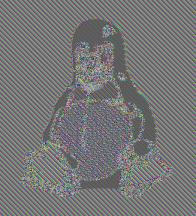
\includegraphics[width=\textwidth]{Figures/Tux_ecb.jpg}
    \caption{Encrypted using ECB mode}
    \label{figures:tux_ecb}
  \end{subfigure}
  \caption[ECB in practice]{ECB in practice. The original image was created by Larry Ewing using GIMP.}
  \label{figures:ecb_in_practice}
\end{figure}

The other is called Counter mode (CTR).
In this mode the block cipher itself does not encrypt the plaintext.
Instead it is used to produce a pseudo-random sequence of bits, in chunks equal to one block, which is then xor'ed with the plaintext.

To produce the $i$-th chunk $s_i$, it "encrypts" the number $i$ with the provided key:
\[
  s_i = E(k, i)
\]

As a result, a bit stream is generated as shown below:

\[
  S = s_1 \Vert s_2 \Vert \dots \Vert s_n
\]

And the resulting ciphertext is:

\[
  C = m_1 \oplus s_1 \Vert \dots \Vert m_n \oplus s_n
\]

To decrypt, one can generate the same bit stream and xor it again with the ciphertext:

\[
  M = c_1 \oplus s_1 \Vert \dots \Vert c_n \oplus s_n
\]

Notice that this means that we use the encryption algorithm of the block cipher both for encryption and decryption.

Counter mode is a secure mode of operation suitable for use in production.
It also has a nice property called malleability, but more on that later.


\section{Message Integrity}

We now know how to keep a message secret.
Another major cryptographic problem is that of message integrity.
How can we be sure that a message we are reading came from who we think it did?

But why is this even necessary?
Since only the sender and the receiver have the secret key, only they should be able to construct valid ciphertexts.

Well, in general this is not correct.
Let's consider again the case of a block cipher used in CTR mode.
Remember that in this mode the block cipher is not directly used for encryption.
Instead it is used to generate a pseudorandom sequence of bits.
This sequence is then xor'ed to the plaintext and the result is the ciphertext.

Now let's see what will happen if a bit of the ciphertext is flipped, and we try to decrypt it.
Suppose $m_i$ and $c_i$ is the $i$-th bit of the plaintext and ciphertext respectively. $s_i$ is the $i$-th bit of the pseudorandom sequence produced during the CTR mode encryption process.
The follow relation holds:

\[
  m_i = c_i \oplus s_i
\]

Flipping a bit means taking its complement.
This means that the new plaintext bit $M_i$ will be:

\[
  M_i = c_i\prime \oplus s_i = (c_i \oplus s_i)\prime
\]

This means that an attacker could actually produce valid ciphertexts for plaintexts of his choosing by tampering with already sent messages!
This property is called malleability.

There are many more ways that an attacker could tamper with sent messages besides utilising the malleability properties of an encryption scheme.
This means that we need ways to authenticate our messages before we sent them.

\section{Hash Functions}

Before we tackle that problem we will have a look at hash functions.
These hash functions are algorithms that accept as input some data of arbitrary length and output some value of fixed length.

If this value is computed in such a way that the hash function $H$ satisfies the following properties (as stated in \cite{appliedcrypto}), then we call the function a \emph{cryptographic} hash function.

\begin{itemize}
  \item Pre-image resistance\\[0.2cm]
    For essentially any output value $h$ of the hash function $H$ it is computationally infeasible to find any input $x$ such that $H(x) = h$.

  \item Second pre-image resistance\\[0.2cm]
    For a given input $x$ it is computationally infeasible to find a second input $x\prime$ such that $x \ne x\prime$ and $H(x) = H(x\prime)$.

  \item Collision resistance\\[0.2cm]
    It is computationally infeasibly to find any pair of inputs $x$ and $x\prime$ such that $H(x) = H(x\prime)$\footnote{This and the previous property might seem the same, but notice that in the Second pre-image property $x$ is fixed, while in the collision resistance property it is not}.
\end{itemize}

Notice that collision resistance implies second pre-image resistance.
Likewise second pre-image resistance implies pre-image resistance.

\section{Message Authentication}

For the purpose of message authentication there are two main categories of solutions.
The first category uses a shared secret to create some sort of electronic signature for some data that we want to authenticate.
This type of signature is called a Message Authentication Code.

The second category uses a pair of keys, the private key, known only to the person signing the data, and the public key, known to everybody.
The public key is used to verify the signature.

\subsection{Message Authentication Codes (MAC)}

This case has many similarities with symmetric encryption.
Again we assume that there is a secret value, called the key, known only to the two parties communicating.
We also assume that an algorithm called $MAC$ exists which produces the signature, called the tag or mac.

This algorithm takes two inputs, the secret key $k$ and the message\footnote{This message can be plaintext or already encrypted} $m$ itself.
The algorithm works in a way such that the produced tag $t$ can only be calculated if you know $k$.

\[
  t = MAC(k, m)
\]

When the sending party wants to transmit a message, she calculates the tag and appends it to the message so that she sends $m \Vert t$.
The receiving party can recalculate the tag on his own.
He then checks if the appended tag is the same with the tag that he calculated.
If the two tags are the same then he accepts the message, otherwise he rejects it as it is probably tampered with.

\subsection{Public key signatures}

In this case we have two distinct algorithms.
On is called $Sign$ and is used to produce the signatures.
The other is called $Verify$ and is used to verify data.

The sender generates a tag $t$ using the $Sign$ algorithm:

\[
  t = Sign(priv, m)
\]

where $priv$ is the private key.
He then appends the tag to the message as in the MAC case and transmits $m \Vert t$.

The receiving party then uses the $Verify$ algorithm.
This algorithm accepts as inputs the message $m$, the tag $t$, and the public key $pub$.
Its result is boolean, responding "YES" if the message is verified and "NO" if it is not:

\[
  result = Verify(m,t,pub)
\]

if $result$ is "YES" then she accepts the message. Otherwise she rejects it.

\section{Key Exchange Protocols (KEP)}

The goal of any Key Exchange Protocol is to allow two users to agree on a secret value, known only to them, by exchanging some publicly known information.
This might be counter intuitive at first but as we will see in the next section this goal can be achieved with a very simple construction.

Basically a Key Exchange Protocol is any mechanism that provides two functions.
One of them returns a tuple containing some private and some public information.
The public information returned by that function must be sent to the other user so that he can calculate the secret value.
The other function accepts the public values of the other user and the private values of this user and returns the secret value.

\begin{figure}[H]
  \begin{align*}
    <priv, pub> &= genkey() \\
    secret &= calculate\_secret(priv_i, pub_j)
  \end{align*}
  \caption[The interface of a Key Exchange Protocol]{The KEP interface. $pub_j$ is the public information of user $j$ and $priv_i$ the private information of user $i$.}
\end{figure}

\section{\dhname key exchange}

The \dhname key exchange is, as the name suggests, a key exchange protocol.
It plays a major role in our proposed protocol, since it is a building block of many of its components.
It was introduce by Whitfield Diffie and Martin Hellman in \cite{dhpaper}.

In this section we will examine how this KEP is constructed, and what public values must be exchanged.

First, we remind to the readers the operation of multiplication modulo a number, $\odot$.
We want to multiply two numbers $a$ and $b$ modulo a number $n$, called "the modulo".
This means that we first multiply the two numbers as usual.
Then we calculate the remainder of the result when it is divided by the modulo.
This remainder is the result of the multiplication of those two numbers $a$, $b$ modulo $n$.
This means that if:

\[
  ab = np + r
\]

Then:

\[
  a \odot b  = r
\]
.

In general we will abuse the notation of exponentiation and symbolize:

\[
  a^x \equiv a \odot \dots \odot a = a^x \mod p
\]


These are all the maths needed to understand how the \dhname key exchange works.
To understand why it is also secure is a whole different matter and we will not cover it in this publication.

The \dhname construction supposes that the two users already agree on two values $g$ and $p$ which are publicly known.
The number $p$ must be prime and is called "the modulo" of the protocol.
The number $g$ is called the "generator" and has the property that for every number $k \in [1 \dots p-1]$ there exists a number $l$ in the same range such that $g^l = k$.

The private information for a user is any random integer $x$ such that $ 1 < x < p$.
The public information is $g^x \mod p$ (any exponentiation from now on will be modulo $p$).

The calculation of the shared secret is trivial.
A user $i$, with private information $x$, and public $g^x$, receives the public information $g^y$ of another user $j$.
He then calculates the value $s = (g^y)^x$ which is the shared secret.
Now note that with $i$'s public information, $j$ can also calculate the same value $s = (g^x)^y$.
The calculated value is the same for the two users since:

\[
  (g^y)^x = (g^x)^y = g^{xy}
\]

In algorithm \ref{algo:dh_genkey} we see the $genkey$ function, and in algorithm \ref{algo:dh_calculate_secret} the $calculate\_secret$ function.

From now on, the public and private information of a user will be called public and private keys accordingly.

\begin{algorithm}
  \KwResult{The private and public information needed by the protocol}
  \Begin{
    $x \leftarrow random\_in\_range(1,p-1)$

    $p \leftarrow g^x$

    \Return{$(x,p)$}
  }
  \caption{The $genkey$ function}
  \label{algo:dh_genkey}
\end{algorithm}

\begin{algorithm}
  \KwIn{$g^y$: the public value of the other user, $x$: the secret value of the user calling the function}
  \KwResult{The shared secret, which is known only to the two users}
  \Begin{
    \Return{$(g^y)^x$}
  }
  \caption{The $calculate\_secret$ function}
  \label{algo:dh_calculate_secret}
\end{algorithm}

\section{Person-in-the-Middle attacks}

Although \dhname is a great protocol for calculating shared secrets, it has a grave disadvantage.
Consider the following scenario, where Mallory, an evil attacker can control the network so that she can read, drop, and inject packets:

Alice wants to privately communicate with Bob. She generates a private key $x$ and sends the public key $g^x$ to Bob.

Mallory interjects and copies and then drops the packet containing Alice's public key. She generates a private key $x\prime$ and the public counterpart $g^{x\prime}$. She performs a \dhname exchange with Alice's key and calculates $s_1 = g^{xx\prime}$, since she knows $x\prime$.
She then sends her public key to Bob.

Bob believes that the public key he just received belongs to Alice. He generates his private key $y$, and sends the public key $g^y$ to Alice. He also calculates $s_2 = g^{yx\prime}$ what he thinks is a shared secret known only to him and Alice.

Mallory interjects again to copy and drop the just sent package from the network. She calculates $s_2 = g^{yx\prime}$, again she knows $x\prime$. Then she sends her public key $g^{x\prime}$ to Alice, posing as Bob.

Now Alice receives a public key which she thinks belongs to Bob. Like Bob she calculates the shared secret $s_1 = g^{xx\prime}$ which she thinks is only known between her and Bob.

\begin{figure}
  \centering
  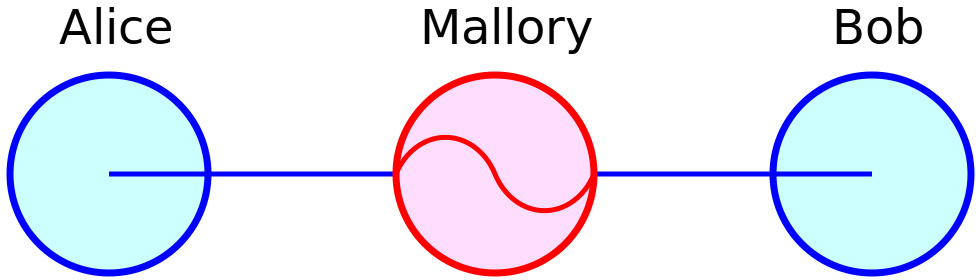
\includegraphics[scale=0.4]{Figures/Person_in_the_middle_attack_cropped.jpg}
  \caption[A Person-in-the-Middle attack]{This figure demonstrates the situation just after Mallory has performed her Person-in-the-Middle attack.}
\end{figure}

The situation now is that Alice and Bob use two different secrets to communicate which are both known to Mallory. Mallory can decrypt any message sent by Alice, for example, since she knows $s_1$.
She then can re-encrypt it using $s_2$ and relay it to Bob.

Neither Alice nor Bob will be able to know that such tampering is taking place and will continue to communicate, thinking that everything is fine.

The above scenario was described with the \dhname key exchange in mind. However any similar situation where a malicious attacker can get between two communicating partners who think they are talking directly to each other is known as a Person-in-the-Middle attack.

\section{\tdhname key exchange}
\label{sections:tdh_key_exchange}
\begin{figure}
  \centering
  \begin{tikzpicture}

  \def \dist {5cm}
  \def \longrad {1cm}
  \def \ephemrad {0.8cm}
  \def \sqrttwo {1.4142}

  \node[draw, circle, minimum size=\longrad] at (0,\dist) {$X$};
  \node[draw, circle, minimum size=\ephemrad] at (0,0) {$x$};
  \node[draw, circle, minimum size=\longrad] at (\dist,\dist) {$Y$};
  \node[draw, circle, minimum size=\ephemrad] at (\dist,0) {$y$};

  \draw[<->, >=latex] ({0 + (\sqrttwo * \longrad / 4)} ,{\dist  - (\sqrttwo * \longrad / 4)})
  -- ({\dist - (\sqrttwo * \ephemrad /4)},{0 + (\sqrttwo * \ephemrad / 4)});

  \draw[<->, >=latex] ({\dist - (\sqrttwo * \longrad / 4)} ,{\dist  - (\sqrttwo * \longrad / 4)})
  -- ({0 + (\sqrttwo * \ephemrad /4)},{0 + (\sqrttwo * \ephemrad / 4)});

  \draw[<->, >=latex] ({0 + \ephemrad/2}, 0) -- ({\dist - \ephemrad/2}, 0);

\end{tikzpicture}

  \caption[\tdhname in a picture]{These are the 3 \dhname key exchanges that are performed in this protocol}
\end{figure}

\tdhname is another key exchange protocol.
It is an improvement of \dhname which introduces negligible overhead in the complexity of the protocol.
With doubling length of the first message containing the public keys of a user, this protocol provides both authentication and deniability.

\subsection{An Overview}

In this key exchange each user has a \dhname longterm keypair.
This should be authenticated to other users to exclude a person-in-the-middle attack, like any other public key scheme.

When Alice wants to communicate with Bob, she generates an ephemeral \dhname key.
Suppose $X$ is her longterm private key and $x$ is her ephemeral private key.

She then sends the tuple $(g^X, g^x)$ to Bob, who upon receiving it does exactly what Alice did. He generates an ephemeral key $y$. Supposing $Y$ is his longterm private key, he then calculates the shared secret $s$ as shown below:

\[
  s = g^{Xy} \Vert g^{xY} \Vert g^{xy}
\]

Notice that an asymmetry exists, in the above calculation.
Should $g^Xy$ got first or should $g^{xY}$?
This can easily be decided by, for example, comparing the longterm public keys.
If $g^X > g^Y$ then:

\[
  s = g^{Xy} \Vert g^{xY} \Vert g^{xy}
\]

and if not:

\[
  s = g^{xY} \Vert g^{Xy} \Vert g^{xy}
\]

And both users will calculate the same secret.

The shared secret generated by the above protocol is forward secret, and authenticated, yet deniable.

It is forward secret since even if someone forces Alice or Bob to hand over their long term secrets, the shared secret cannot be reconstructed.
This is true because to calculate the shared secret, either $x$ or $y$ are needed, and we assume that ephemeral secrets are destroyed after a session finishes.

It is authenticated since to calculate the above secret one needs to know either $X$ or $Y$.

It is deniable since the only values exchanged during the protocol are public keys.

\subsection{The catch}

There is a catch however. Suppose Eve would like to be able to read \emph{some} message that Alice has authored and sent to Bob. What she can do is create an "ephemeral" key $e$. She then starts a conversation with Alice, posing as Bob. She can do this since $Y$ is a longterm key, and $g^Y$ may have previously been publicly exchanged. Alice might respond, create the shared secret and start communicating. Eve does NOT know the shared secret, so she can't read any messages or prove anything, but she might be able to calculate it in the future.

If Eve at some point in the future forces Bob to hand over his long term secrets then she can recreate the shared secret. She can thus read the first message that Alice has tried to send to "Bob" using the shared secret calculated with the phony ephemeral. This is possible since she now knows $Y$ (Bob's longterm secret) and she also knows $e$. This breaks the forward secrecy of the protocol.

This can be easily solved if both Alice and Bob first make sure that they have both arrived at the same shared secret.

Suppose that Alice has calculated the shared secret $s$. She uses that secret to send an encrypted and authenticated message to Bob. That message contains data known to everybody, the word "confirmation" for example. She won't send any further messages unless she receives the same confirmation message from Bob.

On receiving the confirmation message Bob can be sure that Alice has calculated the shared secret.
He then sends a confirmation message himself, so that Alice too can be sure that Bob has calculated the shared secret. Eve could not have sent such a message because she currently doesn't know $Y$, needed for her to calculate $s$.

\section{Message Ordering}
\label{sections:message_ordering}

One difficulty that multi-party chat protocols need to overcome is that of message ordering.
This is confusing at first.
Why would the ordering of the messages be so important?
If a conversation is reordered it shouldn't make any sense.

Unfortunately this is not the case.
To illustrate why message order is important we will examine the so called "ice cream attack".

Suppose that Alice, Bob, and Mallory are chatting in one chat room.
Mallory wants to make Alice believe that Bob is a dangerous criminal.
We assume that she has significant control over the network and can delay packages.
To achieve her goal she does the following:

She sends the message "Who wants some ice cream?" in the chat room.
But she delays the package going to Alice, so that Alice does not receive it yet.
Bob will obviously reply that he wants ice cream.
Let's suppose he sends the message "I do".
Again Mallory will put the package on hold before she delivers it to Alice.
And finally she transmits the message "Who wants to do something illegal?", which she allows to be delivered to both Alice and Bob.
She then allows Bob's message, saying "I do", to go through to Alice.
After that she also allows her original message, saying "Who wants some ice cream?" to also go to Alice.

Now, what did Alice actually see?
First, she saw that Mallory asked who wanted to do something illegal.
And then she saw Bob saying that he does!
In her eyes, Bob is willing to do engage in illegal activities.
Maybe she shouldn't hang out with him any more.

And that exactly is the "ice cream attack".
Can multi-party chat protocols defend against such vulnerabilities?
The problem at hand is generally still open and goes beyond the scope of this publication.
However at section \ref{section:ordering_with_oldblue} we shall briefly examine a proposed solution which is compatible to our protocol.

\chapter{Threat Model}
\label{chapter:threat_model}

\newcommand{\secadv}{$\mathcal{O}$ }
\newcommand{\privadv}{$\mathcal{M}$ }
\newcommand{\conadv}{$\mathcal{T}$ }

Before introducing our mpOTR construction we should define the threat model. We adopt the threat model specified in \cite{mpotr}. First, we introduce the three different types of adversaries. Then, we describe the goals of the mpOTR Protocol regarding each adversary.

\section{The Adversaries}

\subsection{Security adversary $\mathcal{O}$}
This adversary's goal is to read the messages of the chatroom.
Let $T_c^{\hat{X}}$ be the transcript of chatroom $c$ owned by participant $\hat{X}$.
Then, $\mathcal{O}$ is successful, if he can read any message from transcript $T_c^{\hat{A}}$, where $\hat{A}$ is an honest participant, without receiving it from transcript $T_c^{\hat{X}}$ for any participant $\hat{X}$ where $\hat{X} \ne \hat{A}$.
While $\mathcal{O}$ can, both passively and actively, control the network, decrypt messages sent in other chatrooms and even participate in other sessions, he has limited access on the room he wants to attack.
Not only can he not participate in the session under attack, but he also cannot ask for any secret shared between the participants of the specific room.
He has the ability to inject messages of his liking in the chatroom by asking an, otherwise honest, user.
In essence $\mathcal{O}$ is a somewhat formal definition of the notion of IND-CPA attacks in the multiparty setting.

\subsection{Privacy adversary $\mathcal{M}$}

The privacy adversary aims to break the deniability of the protocol.
He is successful if he can prove to a judge $\mathcal{J}$ that a user $\hat{A}$ participated in, read messages from or authored messages in chatroom $c$.

His restrictions are very few.
He can collaborate with $\mathcal{J}$ before the creation of $c$, participate fully in $c$ and even force $\hat{A}$ to reveal his long term secrets in front of the judge.

\subsection{Consensus adversary $\mathcal{T}$}

\subsubsection{Definition of Consensus}

For two participants $\hat{A}$ and $\hat{B}$, consensus is reached on $T_{C_1}^{\hat{A}}$ when $\hat{A}$ believes $\hat{B}$ claims to have a transcript $T_{C_2}^{\hat{B}}$ such that:

\vbox{%
\begin{itemize}
  \label{consensus_def}
  \item $C_1$ has the same set of participants as $C_2$;
  \item $C_1$ and $C_2$ are the same chat room instance;
  \item $T_{C_2}^{\hat{B}}$ has the same collection of messages as $T_{C_1}^{\hat{A}}$;
  \item $T_{C_2}^{\hat{B}}$ and $T_{C_1}^{\hat{A}}$  agree an each message's origin.
\end{itemize}
}

Notice that the above definition is not symmetric.
This means that $\hat{A}$ can reach consensus with $\hat{B}$ without necessarily $\hat{B}$ reaching consensus with $\hat{A}$.

The interpretation of the term "collection of messages" is intentionally left unclear.
This way, each application can handle the ordering of the messages in different ways.

\subsubsection{$\mathcal{T}$'s goal}

$\mathcal{T}$ is successful when he is able to force an honest user $\hat{A}$ to believe that consensus is reached with another honest user $\hat{B}$ when at least one condition from \ref{consensus_def} does not hold.
Notice that only $\hat{A}$ and $\hat{B}$ must be honest.
$\mathcal{T}$ can otherwise control other users as he sees fit.

\section{The Goals of the Protocol}

The protocol must provide some defence mechanisms against all of the above.

The security adversary \secadv can in no way be successful.
The protocol must ensure that no one outside a chat room can read messages authored for it.
This would be a catastrophic failure.

To defend against the privacy adversary \privadv is also crucial.
One might think, that since an attacker can not read messages, it won't make much difference if they are not deniable.
However there are many situations that even evidence that you talked to someone can be incriminating.

If, for example, Ed wanted to reveal to a journalist some evidence about the wrongdoings of a state organization and did that in a non deniable manner then he would be busted.
The correlation between him contacting the journalist and the subsequent release of the information he revealed would mark him as a whistle blower.

Lastly, the consensus adversary \conadv is not strictly cryptographic but is of no less importance.
If an attacker could manipulate the transcripts of two different users, but then convince them that they have received the same messages he could have quite some power over them.
Every multi-party chatting protocol must ensure that all participants view the same messages\footnote{The order of the messages is also very important but this is an open problem and, while various solutions have been proposed, it is not addressed by this work. See section \ref{sections:message_ordering} for a theoretic approach and section \ref{section:ordering_with_oldblue} for our proposed solution.}.

%\include{Chapters/Chapter4}
\chapter{The mpOTR Protocol}
\label{chapters:protocol}

\section{Pproperties of private conversations}
Following the conventions of the OTR protocol, the term "private" is used to describe the properties of casual real-life conversations. The following four properties are both required in two-party as well as multi-party private conversations:
\begin{description}
\item[Confidentiality] No one else apart from the chat room participants can read the messages exchanged.
\item[Authentication] You are assured that the participants are who you think they are.
\item[Repudiation] The messages sent do not have digital signatures that are checkable by a third party. Anyone can forge messages after a conversation to make them look like they came from you. However, during a conversation, other participants are assured the messages they see are authentic and unmodified. 
\item[Forward secrecy] If you lose control of your private keys, no previous conversation is compromised.
\end{description}

In the context of the multi-party chat room, one more property is required:
\begin{description}
\item[Chat room transcript consistency] All participants share the same view over the messages exchanged in a given chat room.
\end{description}


\section{High level protocol overview}
\begin{algorithm}[H]
  \label{algorithms:mpotr_algo}
  \KwIn{$\mathcal{P}$ : participants list}
  \KwResult{Executes a run of the mpOTR protocol}
  \Begin{

    $sid$ := Offer($\mathcal{P}$)
    
    $\mathcal{S}$ := DSKE($sid$, $\mathcal{P}$)
    
    $\mathcal{K}$ := GKA($sid$, $\mathcal{S}$, $\mathcal{P}$)
    
    $\mathcal{A}$ := Attest($sid$, $\mathcal{S}$, $\mathcal{P}$)
    
    \If{$\mathcal{A}$ $\neq$ "OK"}{
      \Return{"Error"}
    }

    $\mathcal{T}$ := Communication($sid$, $\mathcal{K}$, $\mathcal{S}$, $\mathcal{P}$)
  
    $c$ := Shutdown($sid$, $\mathcal{T}$, $\mathcal{S}$, $\mathcal{P}$)
    
    \If{$c$ = "consensus"}{
      \Return{"OK"}
    }
    \Else{
      \Return{"Error"}
    }
  }
  \caption{The mpOTR protocol}
\end{algorithm}

In Algorithm \ref{algorithms:mpotr_algo} we illustrate high-level overview of the protocol. The whole protocol has been divided into sequential phases, which we call sub-protocols. The first four of them (Offer, DSKE GKA and Attest) are responsible for setting up all the needed parameters, for the private communication to take place. The Communication sub-protocol is the one that governs the actual private group conversation. Finally, the Shutdown sub-protocol is responsible for every action that needs to be done before ending each private session. We briefly describe the function of each sub-protocol below.

During the Offer sub-protocol, the participants create a Session ID, $sid$. This is a unique (with high probability) number identifying the session. The Offer sub-protocol is described in more detail in \ref{subsections:offer}. 

During the DSKE sub-protocol, each participant creates an association table $\mathcal{S}$ which maps each participant to the signing key he is going to use for this session. Each participant generates an ephemeral signing key, that she will be using in order to sign her messages during this session. This way she ensures her messages are authenticated. Then, every participant exchanges their ephemeral signing keys with every other participant, using a Deniable Authenticated Key Exchange (DAKE) algorithm. When all exchanges have taken place, every participant has created $\mathcal{S}$. The ephemeral signing keys to be used in this session are deniable. The DSKE sub-protocol and the DAKE are described in more detail in \ref{subsections:DSKE}.

During the GKA sub-protocol, the participants generate a shared key $\mathcal{K}$ that will be used to derive encryption keys. The derived keys, in turn, will be used to encrypt the messages during this session. The GKA sub-protocol is described in more detail in \ref{subsections:gka}

During the Attest sub-protocol, the participants authenticate $sid$ and ensure that they agree on $\mathcal{S}$. The Attest sub-protocol is described in more detail in \ref{subsections:attest}. 

During the Communication sub-protocol, the actual private conversation takes place. The users use $\mathcal{K}$, ephemeral signing keys, and $\mathcal{S}$, in order to encrypt and authenticate their messages. When this phase is finished, a transcript of the chat room $\mathcal{T}$ is returned, which contains all the messages of the chatroom, by participant. The Communication sub-protocol is described in more detail in \ref{subsections:communication}. 

During the Shutdown sub-protocol, the participants determine if $\mathcal{T}$ is consistent, and reveal their ephemeral signing keys. If the transcript is indeed consistent we say that consensus has been reached. The revelation of the ephemeral signing keys adds to the deniability property of the protocol, in the same manner the key revelation in OTR protocol does. However, it’s an optional feature, since the signing keys are deniable in the first place. The Shutdown sub-protocol is described in more detail in \ref{subsections:shutdown}. 


\section{Sub-protocols}

\subsection{Offer}
\label{subsections:offer}
During the first phase of the setup procedure, which we call "Offer", the participants calculate a unique Session ID, called $sid_i$. This is a value that will be used to distinguish the current session between other sessions created by the same set of participants.

Each participant $\hat{X}$ chooses a random 256-bit value $x_{\hat{X}}$, which is his contribution to the $sid_i$. We define $sid_i$ as the SHA-512 hash of the serialized ordered list that contains every participant's contribution.

Each offer message contains the sender's contribution along with his position in the participants list.

The participant who wants to initiate the mpOTR protocol, broadcasts an offer message. Once a participant receives an offer message:

\begin{itemize}
	\item[]He checks if the sender's position contained in the message matches his actual position, if not, he rejects the message.

	\item[]He checks if he has already received an offer message from the sender, if so, he rejects the message.

	\item[]He checks if he has already broadcast his own offer message. If not, creates and broadcasts his own offer message.

	\item[]He checks if he has received every participant's contribution. If so, he calculates the $sid_i$ and proceeds to the next setup phase.
\end{itemize}

Notice that offer messages are not authenticated and hence $sid_i$ must
be verified \emph{after} the participants have exchanged signing keys, as described in \ref{subsections:attest}.


\subsection{Deniable Signature Key Exchange (DSKE)}
\label{subsections:DSKE}
In \cite{mpotr} a construction for a DSKE is proposed. Given a deniable Authenticated Key Exchange (denAKE), two participants of the chat can generate a deniable and authenticated shared secret. With that secret they can exchange their ephemeral signing public key in an encrypted and authenticated fashion, using symmetric algorithms.

This is done for every pair of participants. After that, they will all have created an association table, which associates each participant with their signing key. Afterwards, the participants must make sure that they all have constructed the same association table. This is done by each participant
transmitting the hash of the association table (which is sorted in lexicographical order according to each participant's username). The hash is signed by the ephemeral signing key.

Each participant must verify the signatures in each hash received and also make sure that each hash is the same with the one he has calculated. If everything checks out, then he is assured that the association table is the same.

\subsubsection{denAKE}
In \cite{mpotr} no denAKE is specified. We propose the following protocol:

\begin{itemize}

	\item[] Each participant generates a private/public Diffie-Hellman keypair $(A_i, g^{A_i})$, which will be used as a longterm key to idenitfy him to other participants. This
is done only once, when a member first used the protocol, then the key remains
the same for subsequent runs of the protocol.

	\item[] To initiate a denAKE, each participant creates an ephemeral Diffie-Hellman keypair
		$(a_i,g^{a_i})$ used only in this run of the protocol (he uses however the same ephemeral key
		to communicate with all the participants).

	\item[] Then he broadcasts the public components of the longterm and ephemeral keys to
		all chat participants in the tuple $(g^{A_i}, g^{a_i})$. We shall call this
		message a "Handshake Message".

	\item[] When participant $i$ has received a handshake Message $(g^{A_j}, g^{a_j})$ from some
		other participant $j$, she can compute the shared secret, as specified by the triple
		Diffie-Hellman protocol. This secret is $g^{a_ia_j} || g^{A_ia_j} || g^{A_ja_i}$
		.

	\item[] After computing the shared secret she encrypts and mac's a magic number and sends it
		to the other party. This is done to verify that the other party has indeed generated
		the same shared secret and is not an adversary trying to break the forward secrecy
		property of triple Diffie-Hellman, see \ref{confirm_message_explain}. We shall call
		this message a "Confirm Message".

	\item[] When she herself has received the corresponding Confirm Message she is assured that
		the shared secret can be safely used and there is no foul play. Now she
		encrypts-then-macs her signing public key and sends it to the other party. This
		message is called a "Key Message"


	\item[] When a key message is received he first verifies the message using the same mac.
		If the tag checks out he decrypts the key and adds it in the association table.
\end{itemize}

In figure \ref{den_ake_schematic} a schematic description of the protocol is provided.

\paragraph{Order of the concatenation}
When the shared secret is calculated, three values must be concatenated. Since
concatenation is not commutative the two parties must agree on the order that the
concatenation happens.

This is achieved by compare the values $g^{A_i}$ and $g^{A_j}$. If
$g^{A_i} \le g^{A_j}$ then the shared secret is $g^{a_ia_j} || g^{A_ia_j} || g^{A_ja_i}$
If not then the shared secret is $g^{a_ia_j} || g^{A_ja_i} || g^{A_ia_j}$. That is, the
value that is generated using the highest public key takes precedence during the
concatenation.

In the overview of the algorithm above, it was silently assumed that
$g^{A_i} \le g^{A_j}$.

\paragraph{The need of a confirmation message}
\label{confirm_message_explain}
A confirmation message is needed if want to have forward secrecy in this exchange.
We must make sure that we are really speaking with the intended participant. Consider
the following scenario.

An adversary, Eve, creates an ephemeral keypair $(b, g^b)$. Then he poses as Bob to Alice,
and broadcasts a handshake message containing $(g^B,g^b)$ where $g^B$ is Bob's
public longterm key.

After Alice receives the handshake message she can construct the shared secret. Eve
however cannot construct the secret since she does not know Bob's longterm
private key. If Alice starts sending data before confirming that the other party
has indeed arrived at the same secret she is under the danger to lose the forward
secrecy property for all messages she sends with the secret.

Indeed the only reason Eve can't construct the secret that Alice calculated, is
that she doesn't have Bob's longterm private key. This of course means that if
she somehow gets a hold of this key, she can decrypt some messages. This situation
of course does not satisfy the forward secrecy property.


\subsubsection{Properties}

Triple Diffie-Hellman is a protocol that is a) authenticated b) forward secret
and c) deniable.

It is authenticated, because the shared secret can only be calculated by someone
only if he posses one of the longterm private keys (and the corresponding ephemeral
of course).

It is forward secret, because once the ephemeral key has been destroyed, it is
impossible to reconstruct the shared secret even when the longterm
private key is compromised.

It is deniable, because the only values that are exchanged during a protocol run
are the two public keys that a participant will use. Nothing is signed, which means
that nothing can be used to prove that someone took part in a conversation.\\[0.5cm]

Another property of this protocol that comes for free is its very fast key generation
as, basically, any random number can be used as a secret key.

Thus Triple Diffie-Hellman satisfies the properties required in \cite{mpotr} and
can be used as a denAKE.

\begin{figure}[t]
  \fbox{%
    \pseudocode{%
      \textbf{Alice} \< \< \textbf{Bob} \\[][\hline]
      \text{ Choose a random number $x \in Z_p^*$ }\< \< \\
      \< \sendmessageright*{Send \ \left(g^x,g^X\right)} \< \\
      \< \< \text{ Choose a random number $y \in Z_p^*$ } \\
      \< \< s = g^{xy} || g^{Xy} || g^{Yx} \\
      \< \< k_1 = KDF_1(s) \\
      \< \< k_2=KDF_2(s) \\
      \< \sendmessageleft*{Send \ \left(g^y,g^Y\right)} \< \\
      s = g^{xy} || g^{Xy} || g^{Yx} \< \< \\
      k_1 = KDF_1(s) \< \< \\
      k_2 = KDF_2(s) \< \< \\
      \< \sendmessageright*{ Send \\ c = AES_{k_1}("confirm") \\ MAC_{k_2}(c)\ } \< \\
      \< \< \text{Verify mac} \\
      \< \< m = AES^{-1}_{k_1}(c) \\
      \< \< \text{Verify m = "confirm"} \\
      \< \sendmessageleft*{ Send \\ c = AES_{k_1}("confirm") \\ MAC_{k_2}(c)\ } \< \\
      \text{Verify mac} \< \< \\
      m = AES^{-1}_{k_1}(c) \< \< \\
      \text{Verify m = "confirm"} \\
      \< \sendmessageright*{Send \\ c = AES_{k_1}(\pk_a) \\ MAC_{k_2}(c) } \< \\
      \< \< \text{Verify mac} \\
      \< \< \text{Add $\pk_a$ to association table} \\
      \< \sendmessageleft*{Send \\ c = AES_{k_1}(\pk_b) \\ MAC_{k_2}(c) } \< \\
      \text{Verify mac} \< \<  \\
      \text{Add $\pk_b$ to association table} \< \< \\
    }
  }
  \caption{The denAKE protocol, where $X$ and $Y$ are the private parts of the long term keys}
  \label{den_ake_schematic}
\end{figure}

\clearpage
\subsection{GKA}
\label{subsections:gka}

During this phase the participants derive a shared secret key $g_k$ to be used
as a symmetric encryption key.

The main idea is to compute a combined Diffie-Hellman-like key for all
participants, which will then be used for encryption.

To do this. each participant in the chatroom generates a private exponent.
The shared base is then raised to this exponent. The key agreement begins
by the initiating participant sending his public key to the next participant.

In each step that follows, the participant who just received a list of intermediate
keys from the previous participant must calculate the next intermediate key list and
forward it to the next participant, until the final participant. These messages
shall be called "Upflow Messages".

During the $i$-th iteration, the corresponding participant receives keys from the
$(i - 1)$th participant. and then sends information to the $(i + 1)$th participant.
When the last participant has received the required information, he computes a)the
shared secret and b) the final intermediate key list and then forwards it back to
all previous participants. This message, containing the last intermediate key list
shall be called "Downflow Message".

The other participants now can also caclulate the shared secret and use it for
encryption, using the intermediate key list.

\subsubsection{Detailed description}
For a more detailed description of the protocol we refer to \cite{mpenc}, however
a pseudocode is provided.\\

Algorithm \ref{upflow_algo} presents an overview of how each upflow message is constructed, using the data received from the previous upflow message.\\

Algorithm \ref{downflow_algo} presents an overview of how the final, downflow message is constructed using the data received from the last upflow message.\\


In algorithm \ref{gka_proto_algo} the two previous algorithms (\ref{upflow_algo} and \ref{downflow_algo}) are used in order to execute a complete run of the gka protocol.\\

\begin{algorithm}[H]
	\KwIn{P : participants list}
	\KwExtraIn {InterKeys : previous intermediate key list}
	\KwExtraIn {X : user's secret key}
	\KwExtraIn {N : next participant}
	\KwResult{Sends the new intermediate key list to the next participant}
	\Begin{
	inter\_key\_list := empty\_list

	inter\_key\_list.append( InterKeys.last\_elem() )

	\ForEach{k in InterKeys}
	{
		inter\_key\_list.append( $k^X$ )
	}

	send( N , P || inter\_key\_list)
	}
	\caption{Upflow Message send algorithm}
	\label{upflow_algo}
\end{algorithm}

\vfill
\begin{algorithm}[H]
	\KwIn{P : participants list}
	\KwExtraIn {InterKeys : previous intermediate key list}
	\KwExtraIn {X : user's secret key}
	\KwExtraIn {N : next participant}
	\KwResult{Sends the downflow intermediate key list to the other participants}
	\Begin{
	inter\_key\_list := empty\_list

	\ForEach{k in InterKeys}
	{
		inter\_key\_list.append( $k^X$ )
	}

	inter\_key\_list.reverse()

	send( N , P || inter\_key\_list)
	}
	\caption{Downflow Message send algorithm}
	\label{downflow_algo}
\end{algorithm}

\begin{algorithm}[H]
	\KwIn{P : participants list}
	\KwOut{The shared secret}
	\KwResult{Executes a GKA and produces the shared secret}
	\Begin{

	prev := get\_previous\_participant()

	next := get\_next\_participant()

	x := gka\_genkey()

	\If{prev == NULL}{
		send\_upflow(P, [G], x, next)
		}
	\Else{
			m = receive\_from(prev)

			\If{ m not valid}{
					return error
			}
			\If{ next != NULL}{
				send\_upflow(P, m.key\_list, x, next)
			}
			\Else{
				final\_key := m.key\_list.last\_elem()

				s := $final\_key^x$

				send\_downflow(P, m.key\_list, x)

				return s
			}
	}

	m = wait\_for\_downflow()

	\If{m not valid}{
		return error
	}

	final\_key := m.key\_list[pos]

	s := $final\_key^x$

	return s

	}
	\caption{The GKA protocol}
	\label{gka_proto_algo}
\end{algorithm}

\begin{figure}[H]
  \begin{minipage}{0.49\textwidth}
    \begin{tikzpicture}[scale=.9]
      \def \n {5}
      \def \ndec {4}
      \def \radius {3cm}
      \def \margin {8} % margin in angles, depends on the radius

      \foreach \s in {1,...,\ndec}
      {
        \node[draw, circle] at ({180 + (360/\n * (\s - 1))}:\radius) {$\s$};
        \draw[->, >=latex] ({145 + 36 + (360/\n * (\s - 1))+\margin}:\radius)
          arc ({145 + 36 + (360/\n * (\s - 1))+\margin}:{145 + 36 + 360/\n * (\s)-\margin}:\radius);
      }
      \node[draw, circle] at ({181 + 360/\n * (\n - 1)}:\radius) {$\n$};
    \end{tikzpicture}
    \caption{This diagram demonstrates the upflow of the intermediate keys}
  \end{minipage}
  \begin{minipage}{0.49\textwidth}
    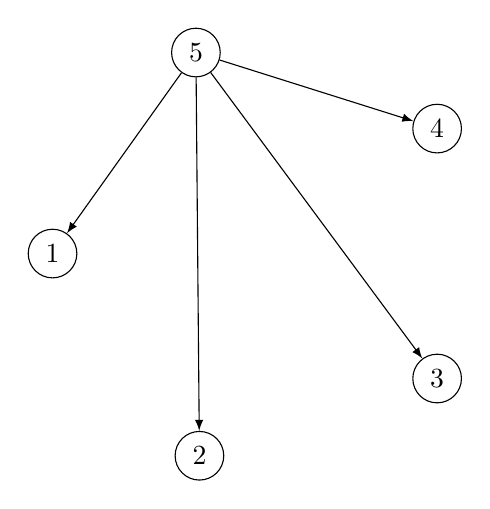
\begin{tikzpicture}[scale=.9]
      \def \n {5}
      \def \ndec {4}
      \def \radius {3cm}
      \def \margin {8} % margin in angles, depends on the radius

      \foreach \s in {1,...,\ndec}
      {
        \node[draw, circle](\s) at ({180 + (360/\n * (\s - 1))}:\radius) {$\s$};
      }
      \node[draw, circle](5) at ({181 + 360/\n * (\n - 1)}:\radius) {$\n$};
      \draw[->, >=latex] (5) -- (1);
      \draw[->, >=latex] (5) -- (2);
      \draw[->, >=latex] (5) -- (3);
      \draw[->, >=latex] (5) -- (4);
    \end{tikzpicture}
    \caption{This diagram demonstrates the downflow of the intermediate keys}
  \end{minipage}
\end{figure}

\subsection{Attest}
\label{subsections:attest}
During this phase the participants must verify that they agree on the $sid_i$,
and the association table as we mentioned in \ref{subsections:offer} and \ref{DSKE}.
This is needed for two reasons. First because $sid_i$ is required before a signing key association table is constructed, and therefore the messages exchanged for the $sid_i$ calculation can not be signed. Second because the participants need to verify that they all have the same view of the association table.

Each participant calculates the SHA-512 hash of the serialized association table and broadcasts an encrypted and authenticated message that contains both the $sid$ and the calculated hash.
To authenticate the message, the sender uses the ephemeral signing key he has now exchanged with the other participants. When each participant has received the attest messages from every other participant she must check two things. She must verify that the hashes of the serialized association table she has received from the other participants are the same with the hash she computed herself. She also must check that all participants have sent their messages using the same Session ID.

Provided that SHA-512 is a cryptographic hash function an attacker cannot find two signing keys association tables with the same hash. This means that he is not able to make two participants believe that they have arrived at the same table when they have not. Also by signing the message with the specific Session ID, a user implicitly verifies that he is using that particular id for this session.

\subsection{Communication}
\label{subsections:Communication}
During the communication phase, the participants can exchange authenticated and encrypted messages using the association table derived from DSKE and the symmetric encryption key $g_k$ derived from GKA.

\subsubsection{Origin Authentication}
For origin Authentication we will use public key encryption methods. This is done because use of symmetric algorithms would require a participant who wishes to send a message to mac the message $n-1$ times, where $n$ is the number of the participants.

\paragraph{Algorithm}
While describing the DSKE we mentioned that an ephemeral signing key is transmitted by each participant to every other, to be used for message origin verification.

For this purpose we make use of the EdDSA algorithm. This algorithm was selected for its fast key generation, since a new keypair must be generated in each protocol run, and its relatively small signature size.

\paragraph{Signing} \label{signing}
The signature generation is the last step taken before sending a message. This
way we can sign all the properties of the message to be sent, like the $sid$ or the
recipient (if any). We also avoid any manifestations of the Cryptographic Doom
Principle, which states that if a protocol tries to perform \emph{any}
cryptographic operation before verifying the signature or mac on a received
message, it will somehow fail catastrophically and lead to doom.

Symmetrically the signature verification is the first thing that happens before
any other operation is performed on the received message (cryptographic or not).

\subsubsection{Encryption}
For encryption a shared secret key is used by all the members. This is not a
problem since the origin authentication is provided by the signatures, and
we obviously don't mind any chat member to read a message or we wouldn't
participate in the chat in the first place. For the actual encryption we
use AES-128 in CTR mode.

The use of the CTR mode however has a small pitfall. We must not let the same
nonce be used twice. This is very difficult to achieve in a distributed setting
like a multi-party chat protocol. Despite this we can solve the problem quite
easily. We maintain our original idea of a shared master key, but we don't use
it directly for encryption. Each participant uses the master key and his id in
the chatroom, in order to compute his "personal" encryption key. This encryption
key for participant $p$ is derived as follows:

\[
    K_e = H(ID_p || Key_m)
\]

Provided that $H$ is a cryptographic hash function, an adversary cannot recover
the value $K$ used for encryption as long as he doesn't know the master key.

\subsubsection{Transcript}
In order to execute the shutdown protocol we need to store the transcript of the chatroom.
In reality a seperate transcript is held for the messages from each participant.
The shutdown protocol will then combine all the different transcripts to determine if consensus has been reached.

The transcript is implemented as a linked list. The list is kept sorted in lexicographic order.
When a message is to be added in a transcript list, the list is searched linearly to find the position the new message should be placed.

When user $A$ sends a message he adds that message to the transcript corresponding to himself.
When he receives a message from user $B$ then he adds that message to the transcript corresponding to user $B$.

\subsection{Shutdown}
\label{subsections:shutdown}
During this phase, the participants end the current session and publish their
ephemeral signing keys, to permit modifying the chat transcript. This adds to
the protocol's deniability property. (Notice though, that the protocol is
deniable without publishing the ephemeral signing keys.)

For a session to be terminated, a "Shutdown Message" is sent.
This message signals to other participants that the shutdown phase should be initiated.
It contains the  hash of all the messages sent by the user sending the "Shutdown Message".
When a user receives a "Shutdown Message", he also sends a "Shutdown Message" containing his own messages hash.
If he has already sent his "Shutdown Message" then he does nothing new.

When one participant has received a "Shutdown Message" from all other participants he can send a "Digest Message".
This message contains a digest of all the messages in the chat-room and is calculated as follows:
\begin{itemize}
  \item[] Sort the participants using their usernames in lexicographic order.
  \item[] For each participant $i$ (in that order) calculate the hash $h_i = H(S_i)$, where $S_i$ is set of all the messages sent by this user (sorted in lexicographic order).
  \item[] Calculate the digest $h = H(h_1 || h_2 \dots || h_N)$, where N is the number of participants.
\end{itemize}

When one participant receives a "Digest Message" from some other participant he checks whether the two of them agree on the chat-room transcript.
He simply compares the digest he computed locally to the one sent by the other participant.
He deduces that consensus is reached only if the two digests are the same.

When one participant has received a "Digest Message" from every other participant he broadcasts an "End Message".
This message signifies that the sender will not user the channel to send any messages anymore.
As a result when a participant receives an "End Message" from all other participants, he is certain that he can release his signing secret key.
Now anyone who intercepts the released key can forge chat-room messages.
However all the participants will no longer accept messages signed with the released secret key, and thus it cannot be used to impersonate its previous owner.


\section{Message consistency in constant space}
In \cite{mpotr} a straightforward approach is followed. In order to check if
each participant has received the same set of messages all the messages from
each user must be stored, and during the shutdown phase be lexicographically
ordered and hashed. While this achieves our purpose it requires $O(M)$ space
where $M$ is the number of messages.

We believe that the same effect can be achieved in constant space by using
cryptographic accumulators. One can find more about this primitive in \cite{accum_def}.

Since such accumulators are collision free but at the same time quasi-commutative,
they are ideal for our purposes. We can feed the accumulator with the incoming
messages in whichever order they arrive at each participant. The quasi-commutative
property guarantees that if two participants have received the same set of messages
then their accumulators will arrive at the same value in the end.

Thus, we have removed the need to store the messages in order to sort them during
the shutdown phase. We only need to store the value of the accumulator which,
of course, is constant.

\section{Participants ordering}
In many cases, the protocol demands some ordering of the participants. For example, in the Offer step of the Setup phase, the sid contributions should be concatenated in some order before hashing them. Same stands for the public signing keys in the association table, during the Attest step. So we define an ordering rule for the participants, that is used whenever an ordering of elements corresponding to participants is needed.

Given that the application provides the mpOTR protocol with a unique name describing each participant, we make the convention that every ordering of the participants list is made lexicographically based on that unique name. We also define the position of the participant, as his position in this order, starting counting from zero (0).

\section{Identity Verification}
The identity of a participant is verified during the DSKE phase.
In order for a participant to be verified the fingerprint of his longterm key must be stored in the known fingerprints file, and be explicitly marked as verified.
In our implementation this file is comma separated and is of the form:

\begin{verbatim}
<account_name>,<protocol>,<buddy_name>,<fingerprint>,<is_verified>
\end{verbatim}

The account name is the "address" of the library user in the form username@host, and is provided by the application.
The protocol is a string that is characteristic of the underlying protocol that the specific account uses.
It is again provided by the application.
The buddy name is the nickname that a user is identified with.
For the time being it is the username part of a users "address".
This implies that the underlying protocol provides addresses which do not change often for a user.
It also means that users from multiple hosts are not allowed or else two users with the same username might conflict.
The above holds for a protocol like jabber for example, but is not the case for protocols like IRC.
As a result our implementation is not fully protocol agnostic at this moment.
Finally the fingerprint is the sha256 hash of the public identity key, and the last field is 1 if the key is verified and 0 otherwise.

This file is read during the plugin start up and initializes the list of all known fingerprints.
When a new chatroom is created, each participant is assigned a list with all known fingerprints used by this participant (from the above list).
When a "Handshake Message" is received the participants known fingerprints list is checked to find (if it exists) a fingerprint matching the currently used public key.
If such a fingerprint is found and it is verified, then the user is verified for this session.
If the found fingerprint is not verified then the participant is not verified.
If no key is found then again the participant is not verified and an entry for this new key is added in the known fingerprints list.

\section{Details of mpOTR Messages}
All mpOTR messages start with the string "?OTR:" followed by the base64 encoded message and then a "." denoting the end of the message.

\subsection{Data Types}
This is how several data types are encoded:
\begin{description}[align=left]
\item [Shorts:] 2 byte unsigned value, big-endian
\item [Integers:] 4 byte unsigned balue, big-endian
\item [Multi Precision Integers:] 4 byte unsigned len, big-endian \\
len byte unsigned value, big-endian
\item [Lists:] 4 byte unsigned len, big-endian \\
len list elements
\item[Hashes:] 32 or 64 bytes of data
\item[CTR-mode counter value:] 8 bytes data
\end{description}


\subsection{Message Structure}
The general structure of mpOTR messages is the following: \\

\begin{bytefield}[bitwidth=0.11111\linewidth]{8}
\bitheader{0-7} \\
\begin{rightwordgroup}{Header}
\bitbox{2}{PV} & \bitbox{2}{MT} & \bitbox{4}{Instance Tag} \\
\wordbox{4}{Session ID (64 Bytes)}
\end{rightwordgroup} \\
\wordbox{4}{Payload} \\
\wordbox{2}{Signature}
\end{bytefield} \\

\begin{description}[align=left]
\item [PV] Protocol Version
\item [MT] Message Type
\end{description}

Offer Messages contain no Session ID in the header, since Session ID has not been established yet Offer and DAKE and Shutdown KeyRelease Messages contain no Signature.

\subsubsection{Offer Message Payload}
\begin{bytefield}[bitwidth=0.11111\linewidth]{8}
\bitheader{0-7} \\
\bitbox{4}{Position} & \bitbox[lrt]{4}{} \\
\wordbox[lr]{1}{Session ID Contribution} \\
\bitbox[l]{4}{} & \bitbox[rb]{4}{} \\
\bitbox[lrb]{4}{}
\end{bytefield}

\subsubsection{DAKE Handshake Message Payload}
\begin{bytefield}[bitwidth=0.11111\linewidth]{8}
\bitheader{0-7} \\
\bitbox{4}{Ephemeral Key Length} & \bitbox[tlr]{4}{} \\
\wordbox[lr]{1}{Ephemeral Key} \\
\wordbox[blr]{1}{$\cdots$} \\
\bitbox{4}{Longterm Key Length} & \bitbox[tlr]{4}{} \\
\wordbox[lr]{1}{Longterm Key} \\
\wordbox[blr]{1}{$\cdots$}
\end{bytefield}

\subsubsection{DAKE Confirm Message Payload}
\begin{bytefield}[bitwidth=0.11111\linewidth]{8}
\bitheader{0-7} \\
\bitbox{4}{Recipient} & \bitbox[tlr]{4}{} \\
\wordbox[lr]{1}{Triple Diffie-Hellman MAC} \\
\bitbox[l]{4}{} & \bitbox[rb]{4}{} \\
\bitbox[lrb]{4}{}
\end{bytefield}

\subsubsection{DAKE Key Message Payload}
\begin{bytefield}[bitwidth=0.11111\linewidth]{8}
\bitheader{0-7} \\
\bitbox{4}{Recipient} & \bitbox[tlr]{4}{} \\
\wordbox[lr]{1}{Triple Diffie-Hellman MAC} \\
\bitbox[l]{4}{} & \bitbox[rb]{4}{} \\
\bitbox[lrb]{4}{} & \bitbox{4}{Key}
\end{bytefield}

\subsubsection{GKA Upflow Message Payload}
\begin{bytefield}[bitwidth=0.11111\linewidth]{8}
\bitheader{0-7} \\
\bitbox{4}{Recipient} & \bitbox{4}{Key List Length} \\
\bitbox{4}{1st Key Length} & \bitbox[tlr]{4}{} \\
\wordbox[lr]{1}{1st Key} \\
\wordbox[blr]{1}{$\cdots$} \\
\bitbox{4}{2nd Key Length} & \bitbox[tlr]{4}{} \\
\wordbox[lr]{1}{2nd Key} \\
\wordbox[blr]{1}{$\cdots$} \\
\wordbox[blr]{3}{$\cdots$} 
\end{bytefield}

\subsubsection{GKA Downflow Message Payload}
\begin{bytefield}[bitwidth=0.11111\linewidth]{8}
\bitheader{0-7} \\
\bitbox{4}{Key List Length} & \bitbox{4}{1st Key Length} \\
\wordbox[lr]{1}{1st Key} \\
\wordbox[lr]{1}{$\cdots$} \\
\bitbox{4}{2nd Key Length} & \bitbox[tlr]{4}{} \\
\wordbox[lr]{1}{2nd Key} \\
\wordbox[blr]{1}{$\cdots$} \\
\wordbox[blr]{3}{$\cdots$}
\end{bytefield}

\subsubsection{Attest Message Payload}
\begin{bytefield}[bitwidth=0.11111\linewidth]{8}
\bitheader{0-7} \\
\wordbox{2}{Session ID (64 Bytes)} \\
\wordbox{2}{Association Table Hash (64 Bytes)} 
\end{bytefield}

\subsubsection{Data Message Payload}
\begin{bytefield}[bitwidth=0.11111\linewidth]{8}
\bitheader{0-7} \\
\wordbox{1}{CTR} \\
\bitbox{4}{Ciphertext Length} & \bitbox[tlr]{4}{} \\
\wordbox[lr]{1}{Ciphertext} \\
\wordbox[blr]{1}{$\cdots$} \\
\end{bytefield}

\subsubsection{Shutdown KeyRelease Payload}
\begin{bytefield}[bitwidth=0.11111\linewidth]{8}
\bitheader{0-7} \\
\bitbox{4}{Key Length} & \bitbox[tlr]{4}{} \\
\wordbox[lr]{1}{Key} \\
\wordbox[blr]{1}{$\cdots$} \\
\end{bytefield}
\chapter{Implementation}
\label{chapters:implementation}

%--------------------------------------------

\section{Summary}
Our primary goal was to design and implement the protocol we specified as a production-grade software, aiming to meet the needs of a wide user base. Of course every user would expect of such a software to offer privacy in communication between two parties too. That said, implementing mpOTR as part of the OTR library was a natural decision. Not only would this result in a complete IM privacy library, but it would, as well, affect an already existing wide user base.

There exist quite a few implementations of the OTR Library, but only two of them have been actually developed by the OTR Development Team. The first one is implemented in C, it's the very first implementation and the most actively developed having 4 major versions with latest release in March of 2016. The other one is implemented in Java, and has only one release in October of 2009. We chose to develop mpOTR as part of the C implementation of the OTR Library.

\section{Designing the Integration}
Integrating a new feature into an existing software is quite a challenge. Ideally, a good design would at least follow the same coding style, make the best possible reuse of the existing code and follow the same design patters. However, after a carefull inspection of the OTR Library source code we realized that following this approach was unfeasible.

First of all, the coding style in OTR Librady source code is inconsistent. Different characters have been used for indentation, there is no standard error handling style, etc. Reusing parts of the existing code was not an option most of the time due to extensive coupling between the various modules. Finally, no specific design patterns had been used in the existing code.

Our approach was rather different. First, we used the coding style used more frequently in the existing code. The code reuse was limitted to the Diffie-Hellman implementation that was the only reusable module of the existing code. As for the design patterns, we decided to use them based on theory.


\section{Design Challenges in C}
A great deal of the callenges a software engineer is going to face when designing a software to be developed in C origins in the lack of literature regarding the Design Patterns. Most of the relative literature, such as the commonly referenced \cite{gofdesignpatterns}, describe the actual implementations of the patterns in the context of an object oriented design.

Given that C is not object oriented language, a developer should be innovative when implementing commonly used design patterns. Fortunately, C is a powerfull language offering the mechanisms to implement almost any design pattern. This power mainly comes from two features, the ability to specify incomplete types in order to achieve abstraction in the sense of information hiding, and the use of \textit{void*} in order to achieve generality as interface and inheritence would do in an object oriented context. The latter must be used carefully, since it could raise the risks regarding type-safety.

The most complete reference of design patterns in C can be found in \cite{patternsinc}. Although it only covers a small number of patterns, it equips the reader with a clear approach of designing patterns when object-oriented techniques are not natively supported by the language. We also used \cite{patternsinc} as a reference for various patterns we implemented.

\section{Design Patterns}
In this section we describe the Design Patterns we utilized in our implementation.

\subsection{First-Class ADT}
First-Class ADT is a pattern that decouples interface from implementation, thus improving encaplulation and providing loose dependencies. We get a definition from \cite{patternsinc}:
\begin{quote}
ADT stands for Abstract Data Type and it is basically a set of values and operations on these values. The ADT is considered first-class if we can have many, unique instances of it.
\end{quote}

Our implementation of First-Class ADTs is based on the paradigm found in \cite{patternsinc}

The header file of each First-Class ADT contains the declaration of a pointer to an incomplete type and the declaration of all functions that the interface constists of. The source file of each First-Class ADT contains the definition of the incomplete type, as a structure and the definition of each interface function.

Instances of the declared pointer will serve as a handle for the clients. This mechanism enforces the clients to use the provided interface functions rather than directly accessing the fields of the structure.

We implemented most of the infrastructure modules as First-Class ADTs, namely \textit{ChatParticipant}, \textit{ChatContext}, \textit{ChatEvent}, \textit{ChatParticipant} and other.

\subsection{Observer}

\subsection{Iterator}

\section{Idioms}

\section{Naming Conventions}

\chapter{The mpOTR Plugin}
\label{chapter:plugin}

In addition to the library we also extended the otr pidgin plugin's functionality.
It now uses the extended capabilities of libotr in order to provide private multi-party chatrooms.

Pidgin is an Instant Messaging (IM) client that is compatible with a wide range of IM protocols.
Since our protocol is protocol agnostic\footnote{This is not wholly true. Our implementation of mpOTR assumes that it can send messages of arbitrary length. This is not true in all IM protocols, IRC being one example.} pidgin users can readily chat securely with their existing contacts.

\section{The plugin workflow}

Allow us now to present in summary the workflow of the plugin.

This is what a pidgin chat conversation looks like when no mpOTR session is taking place.
Notice the mpOTR button on the lower right corner, similar to the OTR button.

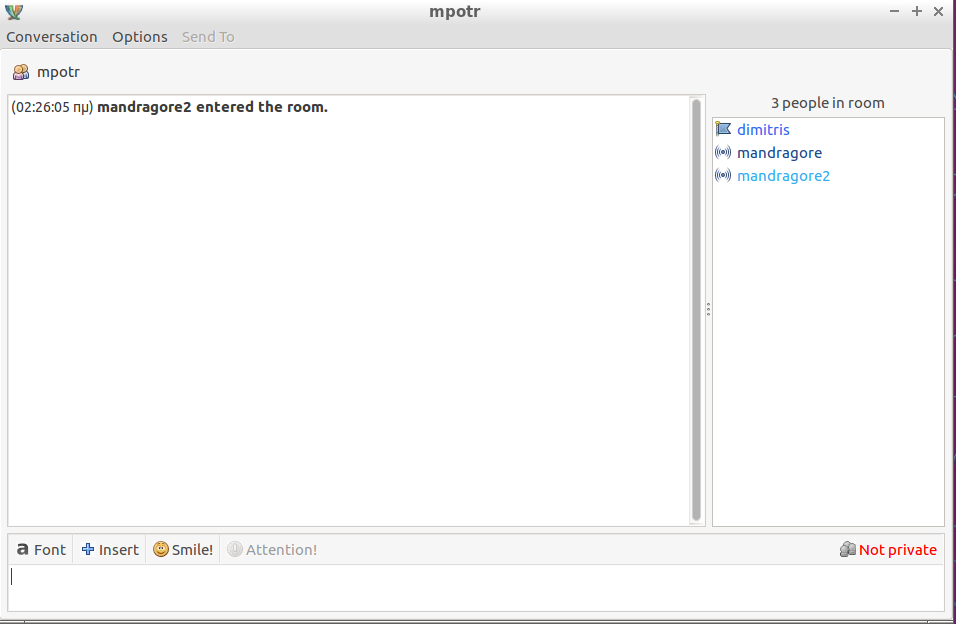
\includegraphics[scale=0.4]{not_started_unverified.png}

By clicking on the mpOTR button a user has the option to start a private conversation.
If he chooses to do so this is what he sees.

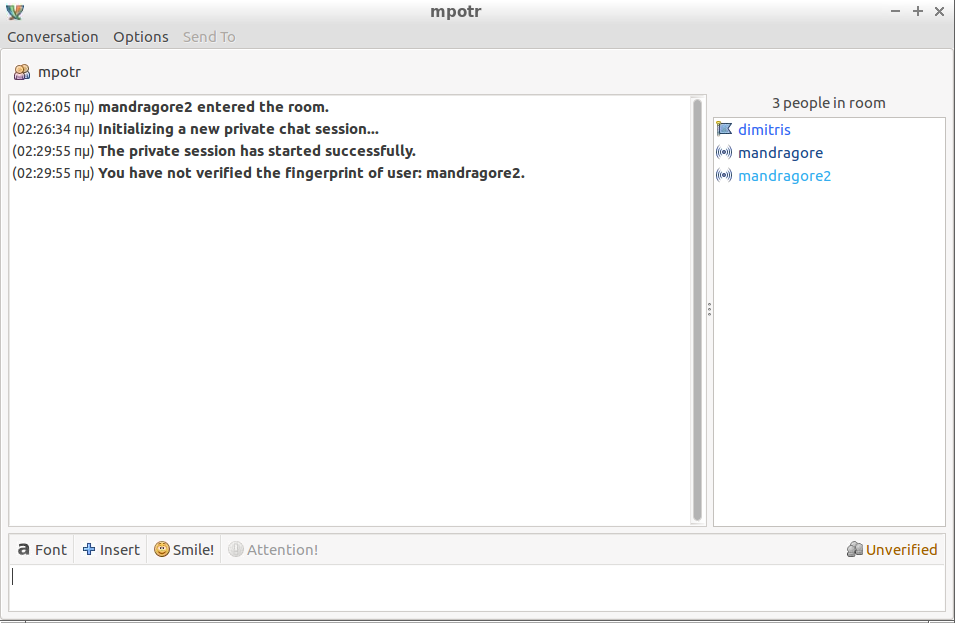
\includegraphics[scale=0.4]{started_unverified.png}

And when some texts are exchanged.

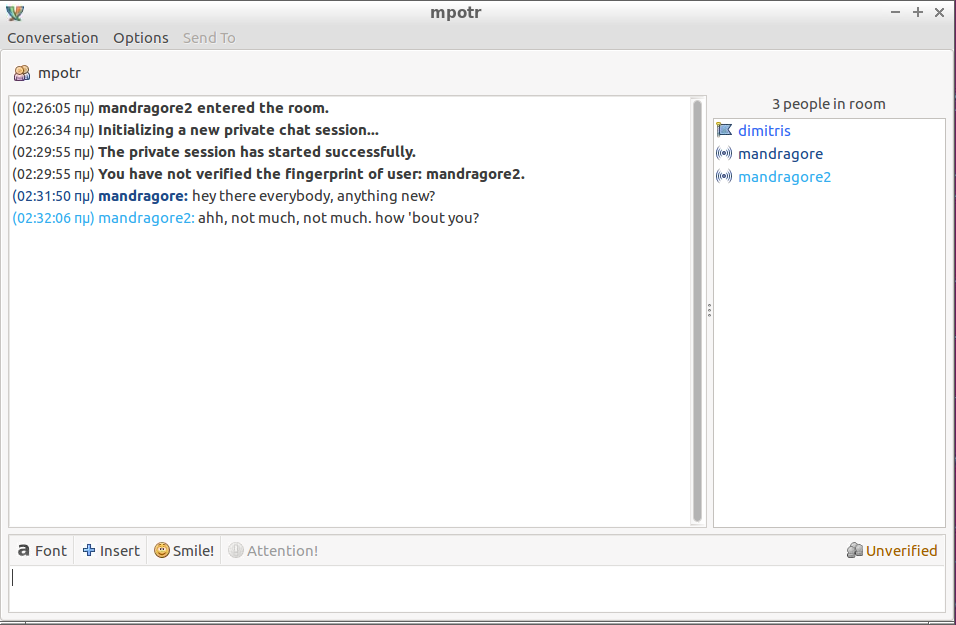
\includegraphics[scale=0.4]{talking_unverified.png}

However, our user (mandragore) hasn't verified another user (mandragore2).
This means that the conversation is unverified.
This is presented to the user in two ways.
First the mpOTR button has a yellow colour and states that the conversation is "Unverified".
And then, the message "You have not verified user: mandragore2".
This message will be displayed for every unverified user.

In order to verify the user mandragore2, our user clicks on the mpOTR button.
Notice how the "Start private conversation" option is now disabled.

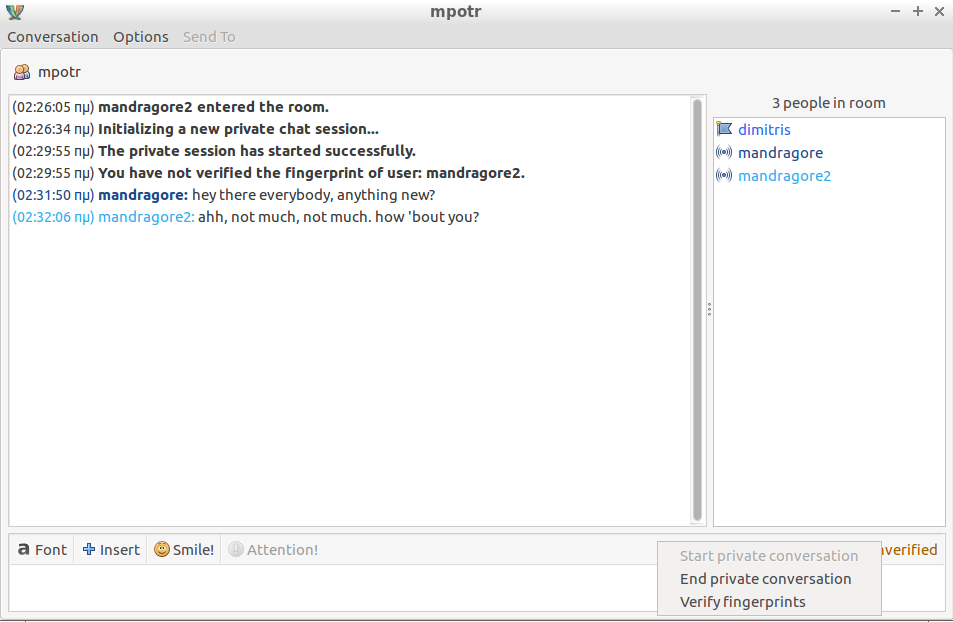
\includegraphics[scale=0.4]{click_mpotr_button_unverified.png}

If he clicks the "Verify fingerprints" option this window opens.

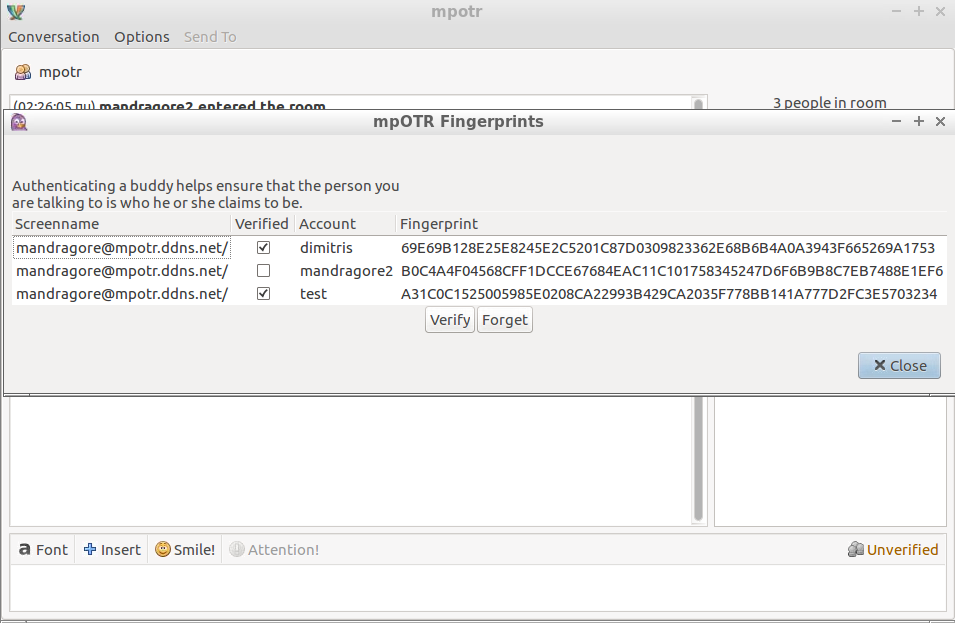
\includegraphics[scale=0.4]{verification_ui_opened_unverified.png}

In this window the user can click on the user he wants to verify and (after he checks the fingerprint) click on the "Verify" button.
The selected user will now be verified.

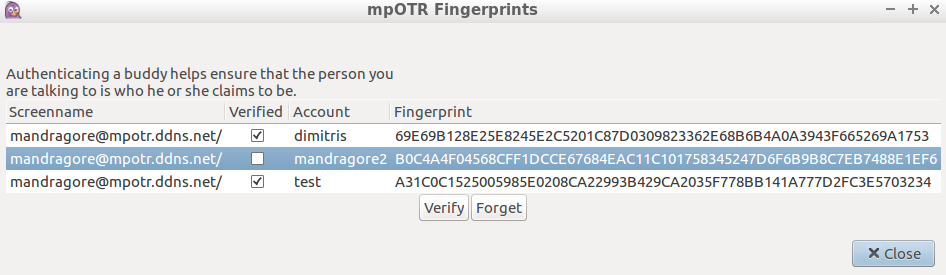
\includegraphics[scale=0.4]{verification_ui_selected_user_unverified.png}

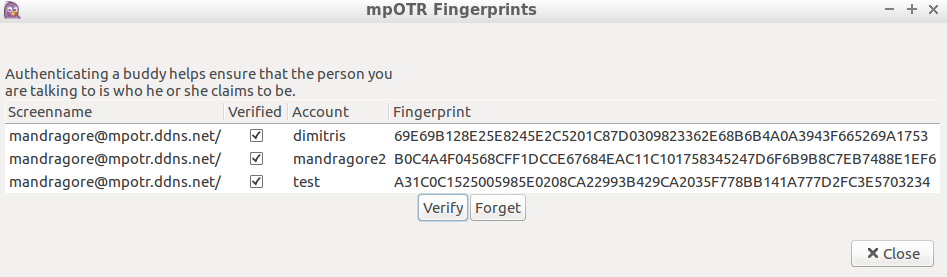
\includegraphics[scale=0.4]{user_verified_unverified.png}

To end the conversation the user clicks on the mpOTR button again and selects the "End private conversation" option.

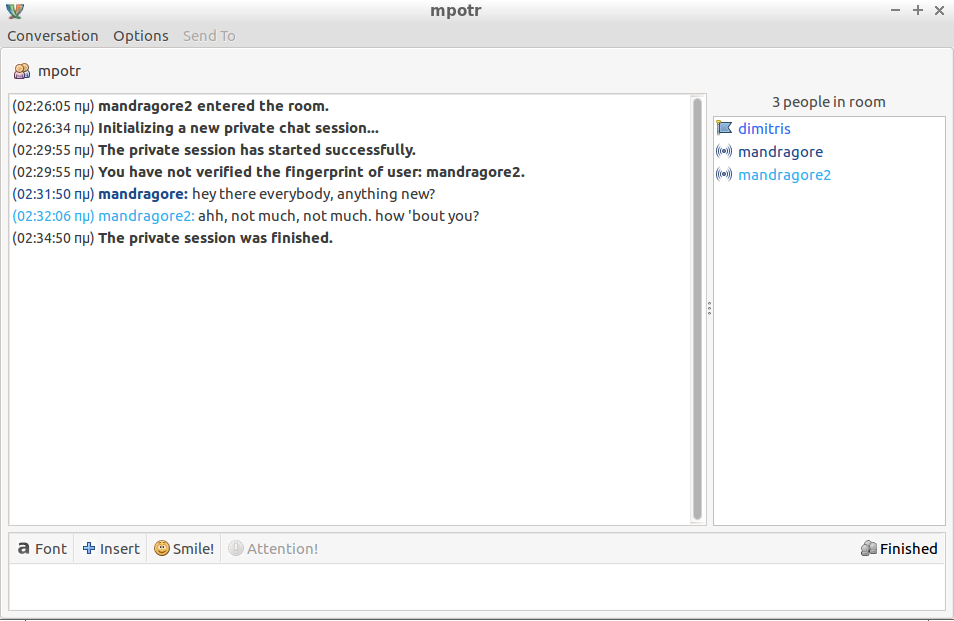
\includegraphics[scale=0.4]{finished_unverified.png}

Now if the user starts another private conversation the new session will be characterised as "Private".

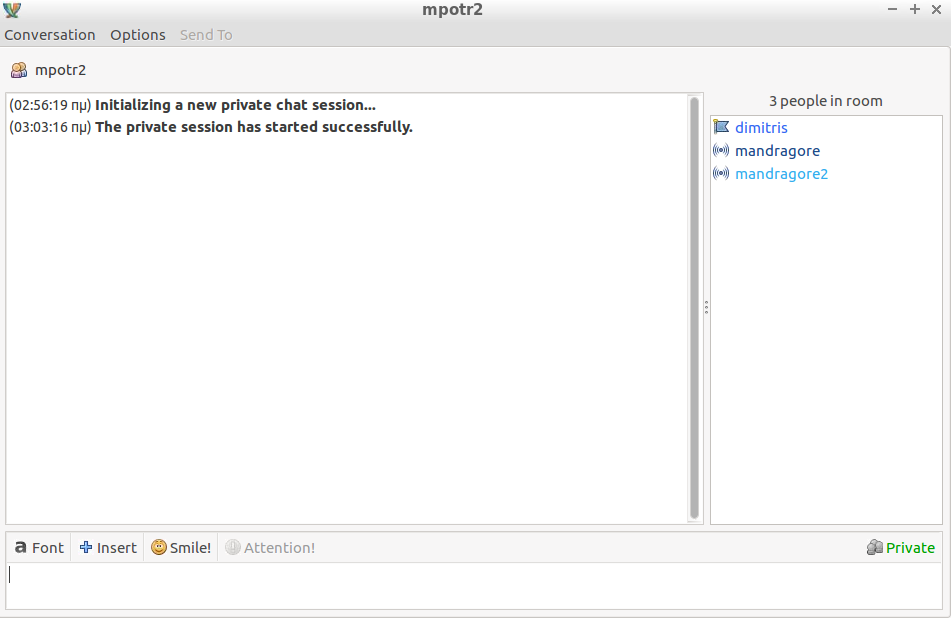
\includegraphics[scale=0.4]{started_verified.png}


\chapter{Related Work}
\label{chapter:related_work}

As we have already stated, end-to-end encrypted instant messaging is a very trending topic in  the crypto community.
Consequently, a plethora of protocols and implementations achieving the above goal exist, the majority of them handling the two-party case.

Here we will present a brief collection of the aforementioned protocols.
Our goal is not to be exhaustive, but rather to give credit to the authors of those protocols.
Either because their ideas gave us inspiration, or because we experienced first hand the difficulties of implementing and designing secure communication applications, and would like to acknowledge their contributions.

\section{Two-party Protocols}

First we will take a look at protocols providing conversations between two parties.

\subsection{Off-the-Record Messaging}

This protocol could not be missing from this section.
It is designed by the same team which authored the original Multi-part OTR paper \cite{mpotr}.

As far as we know it is the first complete protocol to provide end-to-end encrypted Instant Messaging with strong cryptography.
It set the ground for many other protocols and algorithms, like the axolotl key ratchet, which later evolved into the Signal protocol.

\subsection{Vuvuzela}

\noindent\enquote{\itshape We kill people based on metadata}\bigbreak

\hfill {\small Michael Hayden, former NSA director}
\bigbreak

While end-to-end encryption is an essential component for any privacy protecting protocol, it is not perfect on its own.
The metadata can reveal a bunch of crucial information that can be used to even determine the contents of encrypted data.

Vuvuzela \cite{vuvuzela} is a protocol that provides strong metadata privacy that scales.
It utilizes onion encryption (like TOR) to hide metadata.
Messages are sent in rounds, and noise packets are injected in the network in order to defend against traffic analysis attacks.

\section{Multi-party Protocols}

And now let's see some multi-party protocols.

\subsection{Flute}

Flute is a secure multiparty messaging protocol, currently available as a weechat plugin for irc chatrooms.
It provides end-to-end encryption, but does not offer other desirable properties like deniability or chatroom message consistency.

Flute does not provide everything that is needed for a multi-party protocol to be completely secure.
It's simplicity however, allowed it to have a quick implementation, and also provides the challenge to figure out what protocol are crucial in multi-party messaging, and must be added, or do not really enhance the security and should better be left out.

\subsection{Signal}

Signal, developed by Open Whisper Systems, is currently the most complete solution to the multi-party messaging problem.
It is a robust protocol providing all the necessary properties like \emph{confidentiality, authentication, deniability} and \emph{forward secrecy}.
It does not provide \emph{transcript consistency} but the double-ratchet it uses provides some resistance against reordering attacks.

It is available as an Android and iOS application, and for two party conversation can be used through the chrome browser.
Independently from its authors various applications also use it.
What'sApp, Viber, and Facebook Messenger to name a few, are some of the applications that use the Signal protocol to provide secure chats.
Cryptocat is a firefox plugin that closely follows the Signal approach and is completely open source.

\chapter{Future Work}
\label{chapters:FutureWork}

\section{Message Fragmentation}
Some networks may have a message length limitation that is too small to contain an mpOTR message. To solve this problem, OTR has utilized a fragmentation mechanism since version 2.

The OTR fragmentation mechanism is intuitive. On the sender's side, messages are splitted into a sufficient number of pieces N, so that every fragment does not exceed the specified length limit. Each fragment contains a sequence number k, the value of N and the actual piece. The number k indicates the position of the piece in the whole message, starting from 1 and ending to N. On the recipient's side, the fragments are accumulated so that after receiving the piece with its sequence number k equal to N the whole message can be reconstructed.

This fragmentation mechanism works properly as long as the fragments are delivered in-order. In case of out-of-order delivery the algorithm implements a fragment forgetting strategy that finally rejects the message. A more severe problem arises when fragments from different messages are delivered intermixed. Since each fragment contains no information identifying the message it belongs to, the only distinctive information is the number N. In case N contained in a newly received fragment is different than the one contained in the so far accumulated fragments, the so far accumulated fragments are forgotten. But what happens if fragments from different messages splitted into the same number of pieces N are delivered in an intermixed order? Hopefully, the sequence numbers k won't form a valid sequence. In the extreme scenario the latter happens a non-valid message will be reconstructed.

The problems described above are actually unlikely to happen in a two-party communication context. But such a mechanism in a multi-party context would be a bad choice. Even if fragments are accumulated separately for each sender, there is a sporting chance that fragments from different messages sent during the setup procedure will be delivered intermixed. Rejecting such a message would require a restart of the whole setup procedure, and that could possibly occur indefinitely.

\section{Message consistency in constant space}
In \cite{mpotr} a straightforward approach is followed. In order to check if
each participant has received the same set of messages all the messages from
each user must be stored, and during the shutdown phase be lexicographically
ordered and hashed. While this achieves our purpose it requires $O(M)$ space
where $M$ is the number of messages.

We believe that the same effect can be achieved in constant space by using
cryptographic accumulators. One can find more about this primitive in \cite{accum_def}.

Since such accumulators are collision free but at the same time quasi-commutative,
they are ideal for our purposes. We can feed the accumulator with the incoming
messages in whichever order they arrive at each participant. The quasi-commutative
property guarantees that if two participants have received the same set of messages
then their accumulators will arrive at the same value in the end.

Thus, we have removed the need to store the messages in order to sort them during
the shutdown phase. We only need to store the value of the accumulator which,
of course, is constant.

\section{Message Ordering with OldBlue Protocol}
\label{sections:ordering_with_oldblue}

In chapter \ref{chapters:TheoreticBackground} we discussed the problem of message ordering.
We also promised that we would investigate a possible solution to that problem.
In particular we will talk about the OldBlue protocol.
As we shall see this protocol guarantees that the received messages are causally ordered.

\subsection{Why causal ordering}

To understand why the causal ordering is the best we can get let's see what we can and cannot do:
First note that a multi-party chat room is a distributed environment.
This means that there is no central "authority" which can decide if a message came before another.

Also, since we are in a zero trust setting we cannot utilise any values over which the participants have full control, like their local clocks for example.

The only information for which we must trust the other participants is what messages they have seen.
We have no other option on this one as we cannot know if an attacker has actually stopped messages from getting to them or if they are dishonest and lie to us.

As a result the only information about the history of a received message that we can trust (\emph{must} trust actually) is this:
We can only know what message a user admits she has seen, before authoring the received message.
In other words the only thing we can know is which messages might have \emph{caused} the received message.

\subsection{The parent graph}

Using this information on the causal ordering of messages we can construct the parent graph.
This graph will contain all the information about which messages came after some others.
Now lets take a look on the structure of this graph.

Firs of all it is directed.
It retains information on which messages came after other messages.
Since this property is not symmetric our parent graph has directions on its edges.

It is also obvious that this graph is acyclic.
No cycles can exist in this graph since a message cannot possibly cause any of its ancestors.
In other words the edges will always point from the beginning of the conversation towards its end.

In an ideal world, this graph would be a line.
Every user would see  all the previous messages before sending a message, and no two messages would be sent simultaneously.
However this is not the case generally.
Two users may have seen the same set of parent messages and choose to send a message at the same time.
As a result the parent graph will fork, as the same message now has two children.

\subsection{Distributed Parent Graph}

As we said a multi-party chatroom is a distributed environment.
This means that each participant stores and builds a local copy of the parent graph.
To do that each participant attach to each message he sends some information of his local copy so that other participants can find out where they should place his message.

The naive solution would be to include the whole current parent graph in his message but that is obviously infeasible.
Instead much less information is needed.
The actual information that he must send is all the messages in his graph that do not have any children.
This is called the "front" of the graph.

This information is transmitted by appending a list of the hashes of all the "front" messages, to the message to be sent.

\subsection{Dangling messages}

If no re-ordering of the messages occurs then everything works fine.
How do we handle reordered messages however?

The protocol handles two sets of messages.
One is called the delivered set, the other is called undelivered.
When a message is received we check if all of its parents are in the delivered set.
If not then the message is added in the undelivered set and waits there.

If the parents are delivered then the message itself is inserted in the delivered  set and displayed to the user.
After that happens the protocol iterates over the undelivered set and checks if any message is now deliverable (meaning that all of its parents are now in the delivered set).
If it is then, the message is added in the delivered set and displayed to the user.
After that it iterates again over the undelivered set and repeats until there are no deliverable messages.

\section{Group Encryption Key Ratcheting}

Plain OTR has a property called \emph{future secrecy}.
This means that if for some reason the shared secret is compromised, only a few messages in the chat will be revealed to the attacker.
In fact if both of the two participants send a messages after the compromise, then a new key will be generated and the old compromised secret will be useless.

This does not happen in our protocol.
After the GKA is finished the shared secret remains the same until the shutdown phase.

A similar result can be achieved if we run various GKAs one after the other in the background.
We could attach the required upflow and downflow messages in chat messages sent by users during the communications protocol.
If a particular user is away or doesn't participate actively in the chat by authoring messages an chat message can be sent, using a timer interrupt, which will contain the data required for the GKA to continue.
This way the group secret could be ratcheted.

A side-effect of this approach is that the ratcheting of the key will work as a central "clock" of the chatroom.
Messages sent before the change of the secret will no longer be readable by the participants.
This way an attacker would not be able to reorder messages encrypted using two different secrets.


%----------------------------------------------------------------------------------------
%	THESIS CONTENT - APPENDICES
%----------------------------------------------------------------------------------------

\appendix % Cue to tell LaTeX that the following "chapters" are Appendices

% Include the appendices of the thesis as separate files from the Appendices folder
% Uncomment the lines as you write the Appendices

% Appendix A

\chapter{Appendix Title Here} % Main appendix title

\label{AppendixA} % For referencing this appendix elsewhere, use \ref{AppendixA}

Write your Appendix content here.
%\include{Appendices/AppendixB}
%\include{Appendices/AppendixC}

%----------------------------------------------------------------------------------------
%	BIBLIOGRAPHY
%----------------------------------------------------------------------------------------
\printbibliography

%----------------------------------------------------------------------------------------

\end{document}
